\section{Analysis}

\subsection{Description of the simulation}
We consider a set of Monte Carlo cluster simulations, developed with the Monte Carlo
code MOCCA of \citet{2013MNRAS.429.1221H}Hypki et al. 2013 (see also \citet{1998MNRAS.298.1239G} \color{red} is that the right one? \color{black} Giersz et al. 1998). The simulations
include an initial mass function, stellar evolution, primordial binaries, and a
relatively high number of particles, providing a realistic description of the
long-term evolution of \acp{GC} with a single stellar population.

All the simulation had a metallicity of [Fe/H]=$-$1.3 and a Kroupa (2001) \color{red} which one? \color{black} initial
mass function. The first simulation (from \citet{2015MNRAS.454.3150G} \color{red} right one? \color{black} Giersz et al. 2015, kindly shared by the
authors) contain an \ac{IMBH} of \unit[$10^4$]{M$_\odot$} and its initial condition is drawn from a
King model with concentration parameter W$_0 $=6, \unit[6.9]{$\cdot10^5$} initial number of particles,
\unit[95]{\%} of which are binary systems. We consider two snapshots of the simulation on at
10 and one at \unit[7]{Gyr}. We call these snapshots SIM1-IMBH and SIM2-IMBH, respectively.
Other two simulations (from Downing et al. 2010\citet{2010MNRAS.407.1946D}\color{red} this one? \color{black}, kindly shared by the authors), do
not contain an \ac{IMBH} and have an initial number of particles of \unit[5]{$\cdot10^5$} and \unit[2]{$\cdot10^6$}, \unit[10]{\%}
of initial binaries, and initial conditions drawn from a \citet{1911MNRAS..71..460P} model with a
ratio between the initial tidal radius and half-mass radius of 75. We consider a 11
Gyr snapshot for both simulations and we call them SIM3-NOIMBH and SIM4-NOIMBH,
respectively.

We summarize in Table \ref{tab:overview_simulation} the properties of the simulations for the time-snapshots
considered. 


\begin{table}[htbp]
\centering
\begin{tabular}{ c | c | c | c | c | c }
\makecell{Name of the \\simulation} & \makecell{Number of \\ particles} & Total mass [M\(_\odot\)]& \makecell{Mass of the \\ \ac{IMBH} [M\(_\odot\)]}& r\(_\mathrm{m}\) [pc] & Age [Gyr]\\
\hline			
  SIM 1 - IMBH & 1026735 & 3.09\(\cdot 10^5\) & 10102 & 4.13 & 10\\
  SIM 2 - IMBH & 1079376& 3.26\(\cdot 10^5\) & 8902.3 & 3.58 & 7\\
  SIM 3 - NOIMBH & 468627& 1.73\(\cdot 10^5\)& 0 & 7.89 & 11\\
  SIM 4 - NOIMBH & 1851556& 6.70\(\cdot 10^5\)& 0 & 5.41 & 11\\

\end{tabular}
\caption{Overview of the data of the simulations. We show the basic properties of each simulation which are numper of particles, the total mass, the mass of the \ac{IMBH}, the half mass radius and the age. The half mass radius is defined by the radius which includes half of the mass of the whole system.}
\label{tab:overview_simulation}
\end{table}

The output of the simulations relevant for our work are for each star: the position
vector x, the velocity vector v in Cartesian and polar coordinates, mass, luminosity, magnitude b and v band and whether
the star is a binary or not.

\par We compute the half-mass radius \(\mathrm{r_m}\) given in table \ref{tab:overview_simulation} by calculating the distance where half of the mass of the \ac{GC} is inside the sphere of given distance and half of the mass is distributed outside of this sphere. We need it to compare the different simulations since their actual distance is depending on the simulation and is therefore not comparable. 
\\
To get familiar with the simulation we first have a look at the spatial distribution of the stars.
\begin{figure}[htbp] 
\centering
\begin{subfigure}{0.9\textwidth}
	\centering
  	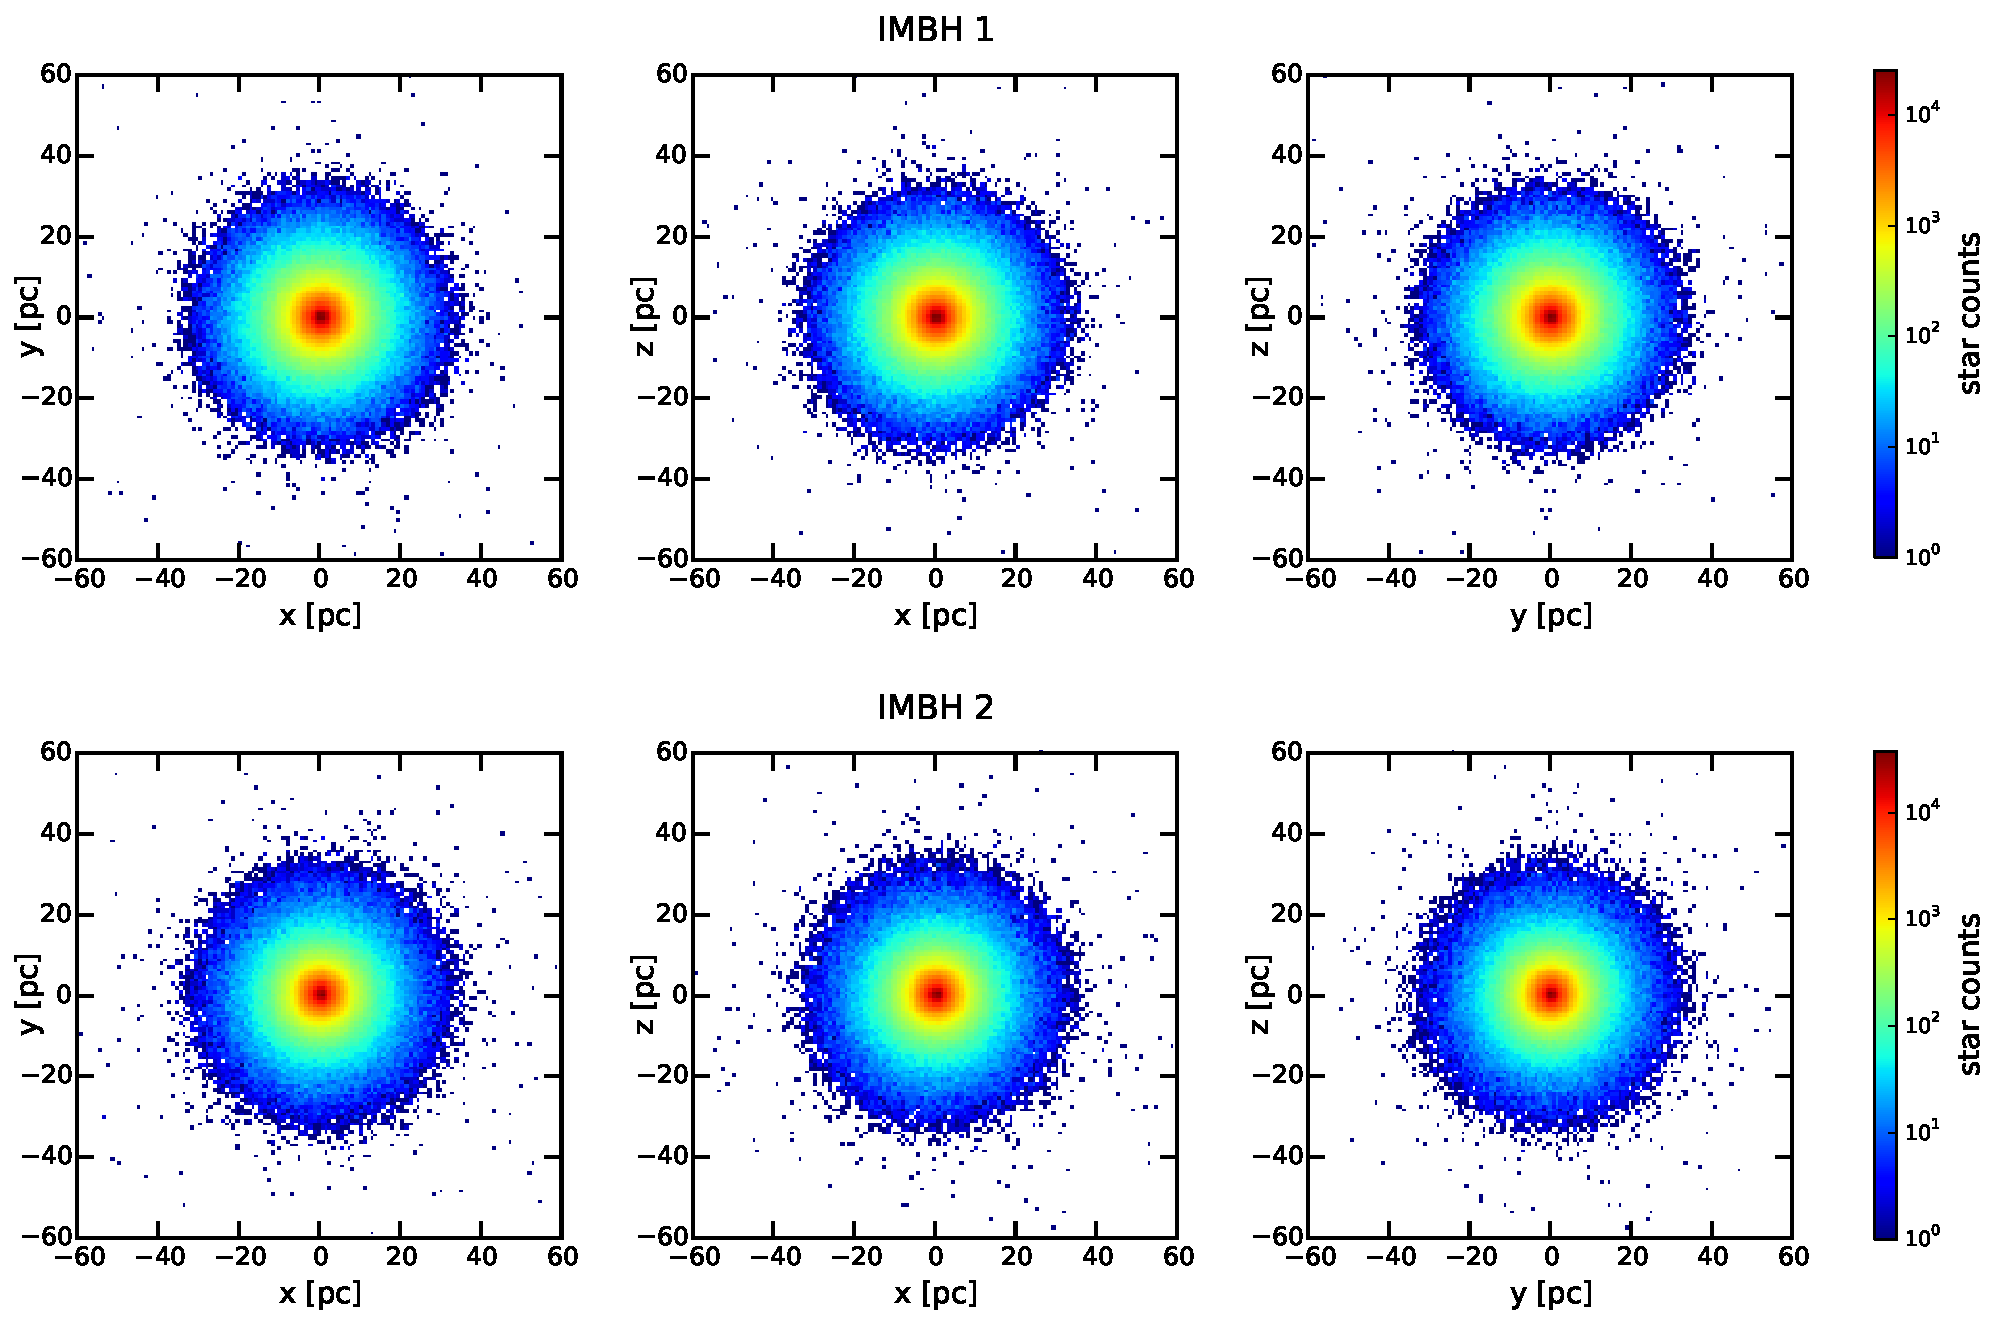
\includegraphics[width=\textwidth]{Plots/position_scatter_plot_IMBH.pdf}
  	\caption{SIM 1 \& SIM 2. The \acp{GC} are spread until \unit[100]{pc} with most of the stars located in the inner \unit[40]{pc}.}
 	\label{fig:pos_scat_IMBH}
\end{subfigure}
\\
\begin{subfigure}{0.9\textwidth}
	\centering
  	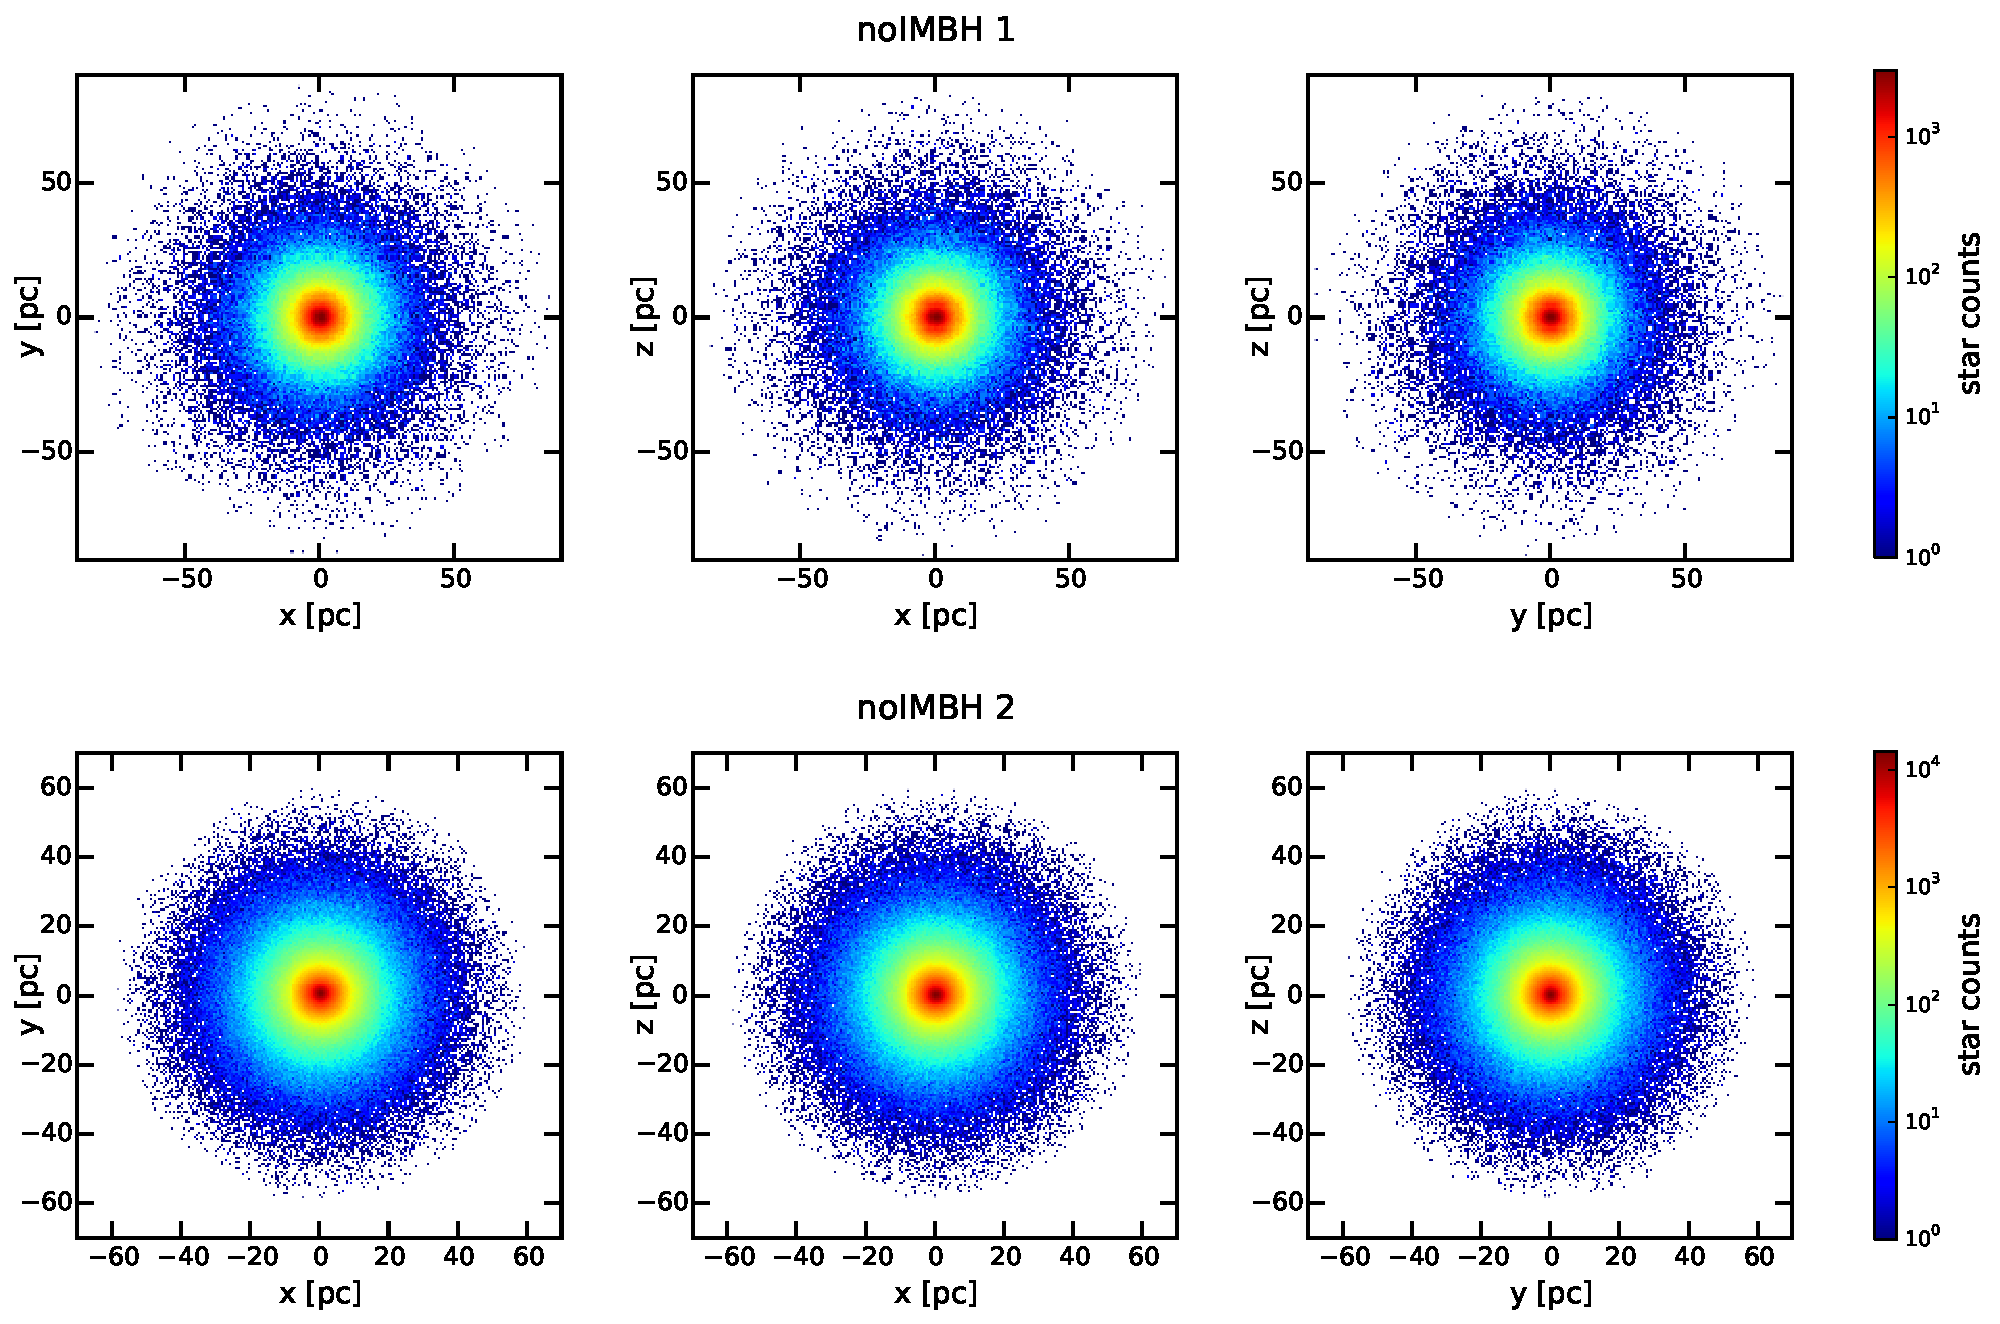
\includegraphics[width=\textwidth]{Plots/position_scatter_plot_noIMBH.pdf}
  	\caption{SIM 3 \& SIM 4. The \ac{GC} is spread until \unit[90]{pc} (SIM3) and until \unit[60]{pc} (SIM4).}
 	\label{fig:pos_scat_noIMBH}
\end{subfigure}

\caption{Spatial distribution of stars in the simulated \acp{GC}. The stars are distributed spherically with most of the stars in the inner part. The stars of the \acp{GC} with \ac{IMBH} are less spread in the outer parts except very few which are far outside. This is simply due to the different initial concentration conditions of the simulations. In the \acp{GC} without \ac{IMBH} the stars in the outer part are less accumulated but the furthermost stars still in the main sphere.}
\label{fig:position_scatter}
\end{figure}

\begin{figure}[htbp] 
\centering
	\begin{subfigure}{0.9\textwidth}
		\centering
	  	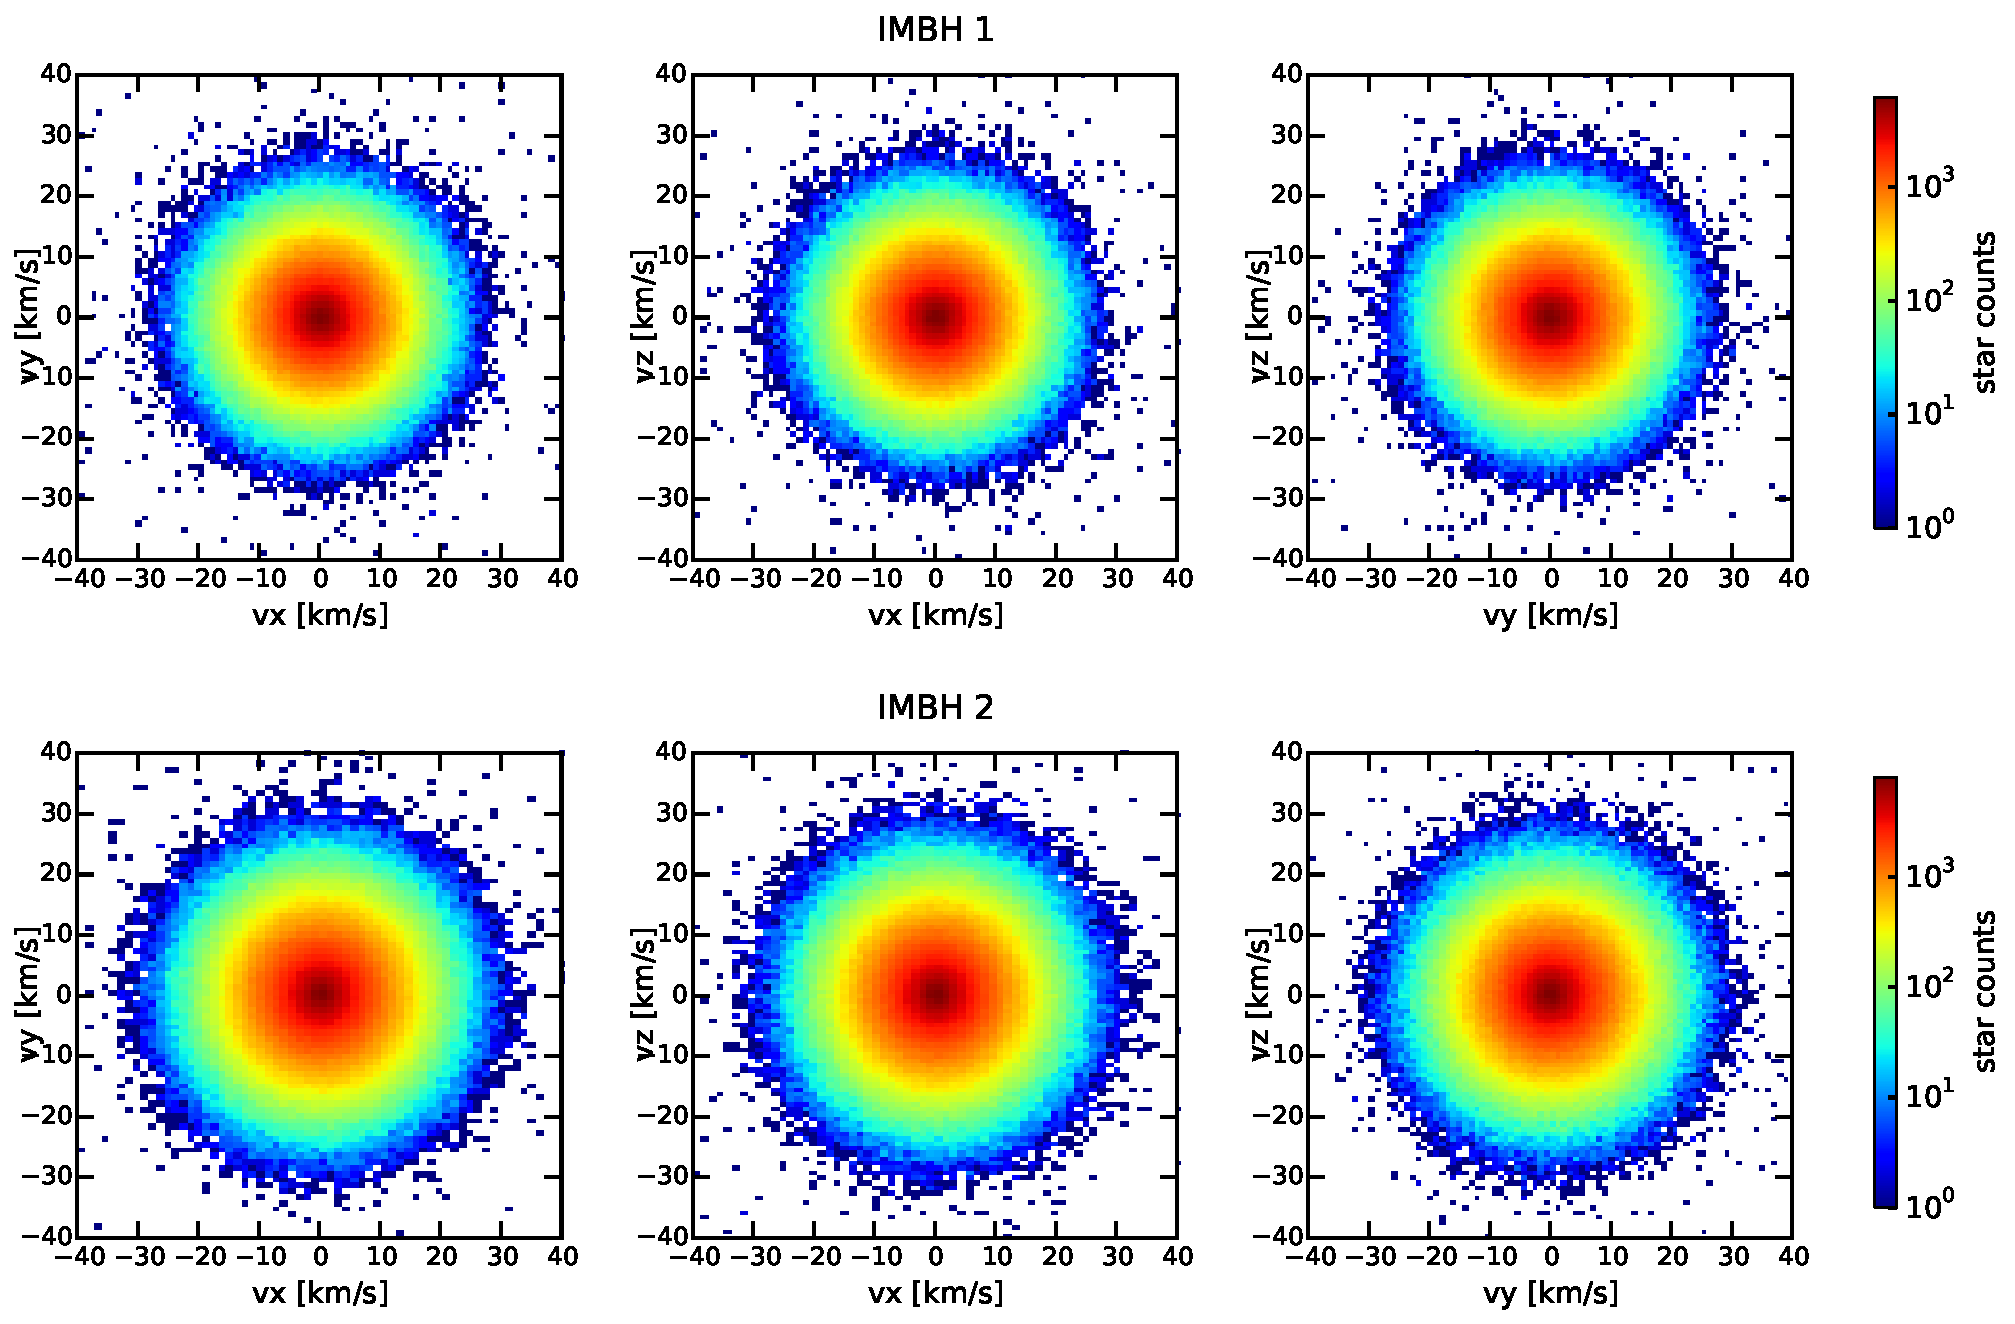
\includegraphics[width=\textwidth]{Plots/velocity_scatter_IMBH.pdf}
	  	\caption{SIM 1 \& SIM 2. The stars' velocities are spread until \unitfrac[120]{km}{s} with most of them reaching \unitfrac[30]{km}{s}.}
	 	\label{fig:vel_scat_IMBH}
	\end{subfigure}
	\\
	\begin{subfigure}{0.9\textwidth}
		\centering
	  	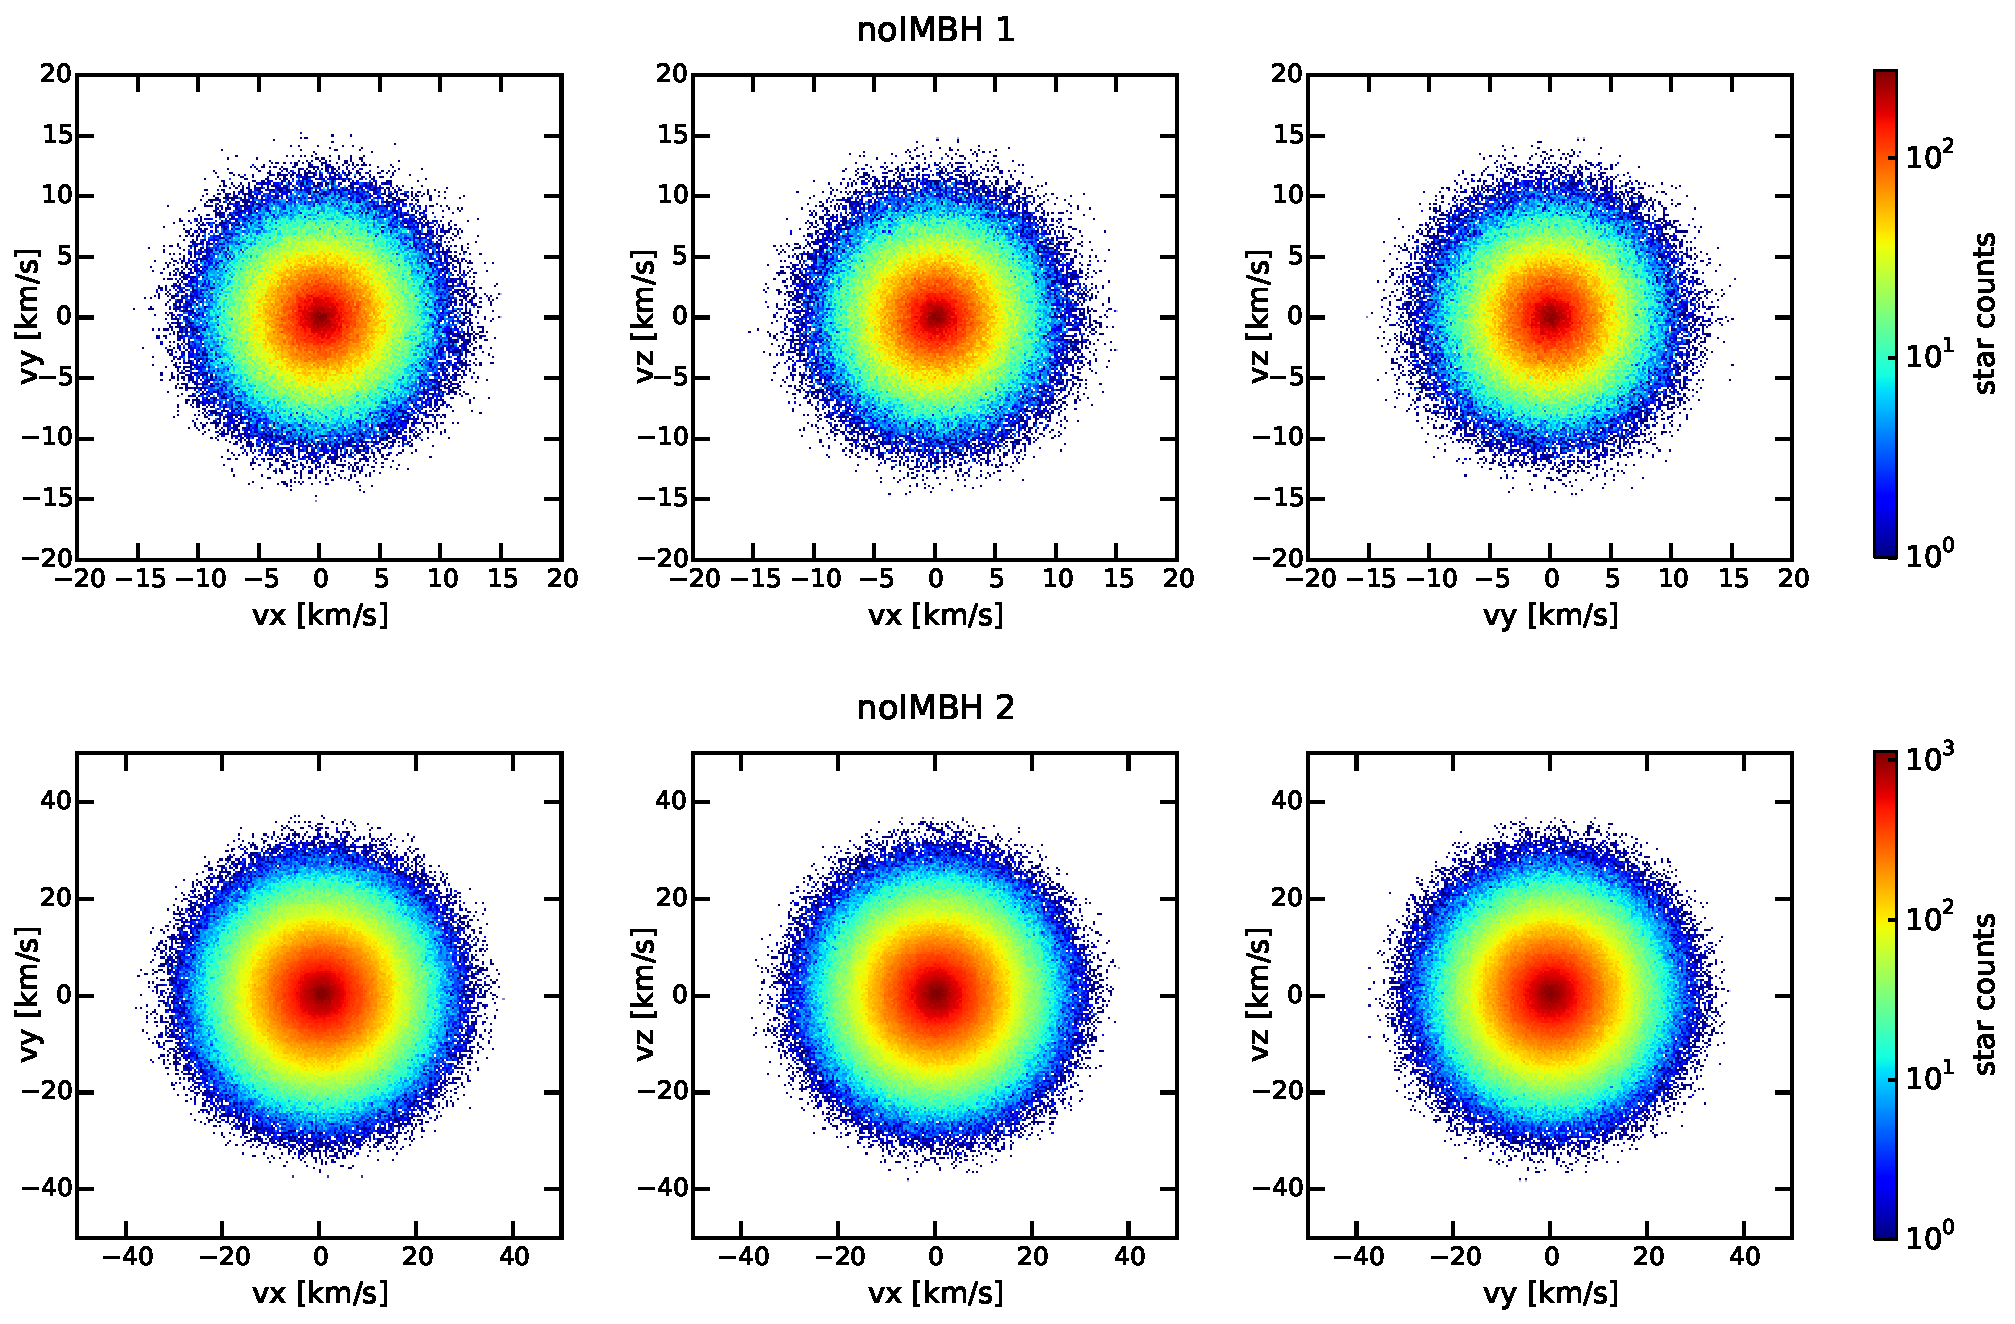
\includegraphics[width=\textwidth]{Plots/velocity_scatter_noIMBH.pdf}
	  	\caption{SIM 3 \& SIM 4. The stars' velocities are spread until \unitfrac[15]{km}{s} for SIM 3 whereas they spread until \unitfrac[40]{km}{s} for SIM 4.}
	 	\label{fig:vel_scat_noIMBH}
	\end{subfigure}

\caption{Velocity distribution of stars in the simulated \acp{GC}. The velocities are isotropically spread around \(\vec{v}=0\). Most of the stars have low or no velocity while a few have high velocities in different directions. There are no overall streaming motions.}
\label{fig:velocity_scatter}
\end{figure}


\subsection{Investigation in color magnitude space}
As mentioned in \ref{cmd_theory} the \ac{CMD} is showing a star's evolution stage dependend on its position. If one do not know age or metallicity of the system isochrones can be fitted on the \ac{CMD}. We plot several isochrones (see section \ref{cmd_theory}) to our \ac{CMD} to determine which one fits best. This will give us the age and the metallicity of the system. 
\begin{figure}[htbp]
\centering
\includegraphics[width=0.7\textwidth]{Plots/cmd_isochrones}
\caption{Color magnitude diagram of SIM 1 overplotted with different isochrones. We recognize how we can determine the age based on the turn off point. This verifies the age and the metallicity of this \ac{GC} of \unit[10]{Gyr} and 0.001.}
	\label{fig:cmd_isochrones}
\end{figure}



\subsection{Investigation in phase space}

First we will investigate the \ac{GC} in phase space for the set of simulations that we will use throughout this work. We will start with the velocity dispersion and the anisotropy parameter then we will have a density profile and from that get the potential. 

\subsubsection{Kinematics}
With equation \eqref{eq:vel_disp} from section \ref{kin_prof_theory} we can calculate the velocity dispersion in each coordinate direction \(\sigma_\mathrm{r},\sigma_\theta,\sigma_\phi\). For every bin we take the same amount of stars and calculate the dispersion along the radius of the \ac{GC}. As radial values we use the average radius of the stars falling in the bins. To compare all simulations we plot the dispersion over the distance in units of the half-mass radius. The half mass radii of the simulations can be taken from table \ref{tab:overview_simulation}. 
\begin{figure*}[htbp]
	\centering
	\begin{subfigure}{0.475\textwidth}
		\centering
		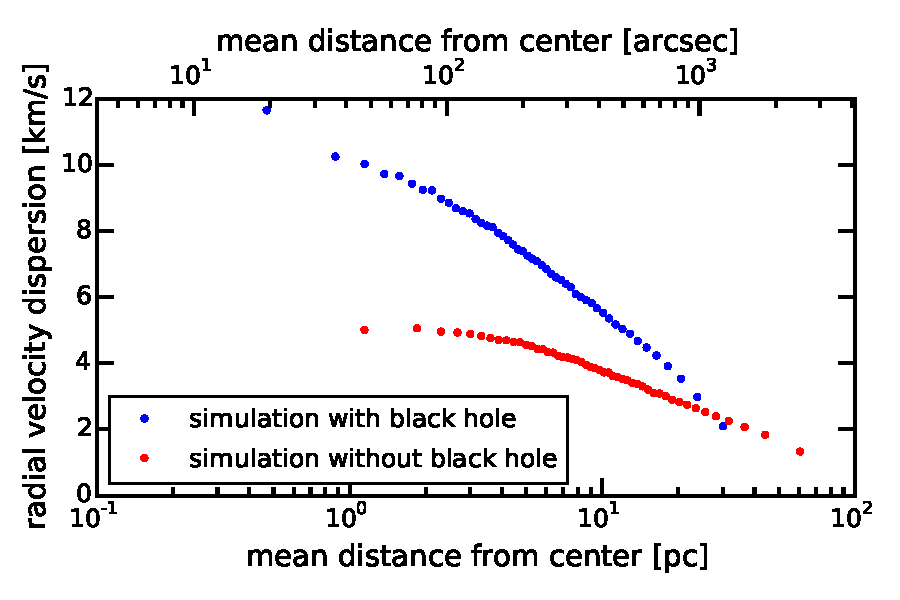
\includegraphics[width=\textwidth]{Plots/radial_velocity_dispersion.pdf}
		\caption{Radial velocity dispersions}
		\label{[fig:radial_vel_disp]}
	\end{subfigure}
	\hfill
	\begin{subfigure}{0.475\textwidth}
		\centering
		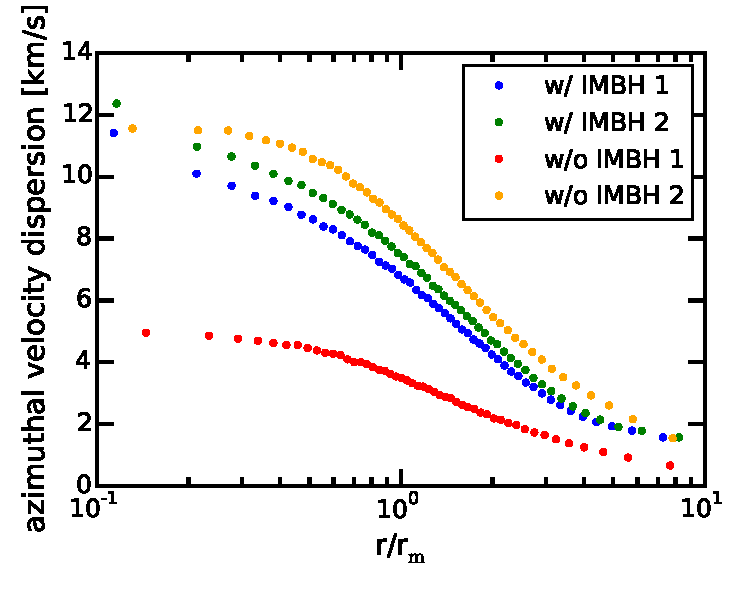
\includegraphics[width=\textwidth]{Plots/azimuthal_velocity_dispersion.pdf}
		\caption{Azimuthal velocity dispersions}
		\label{[fig:azimuthal_vel_disp]}
	\end{subfigure}
	\vskip\baselineskip
	\begin{subfigure}{0.475\textwidth}
		\centering
		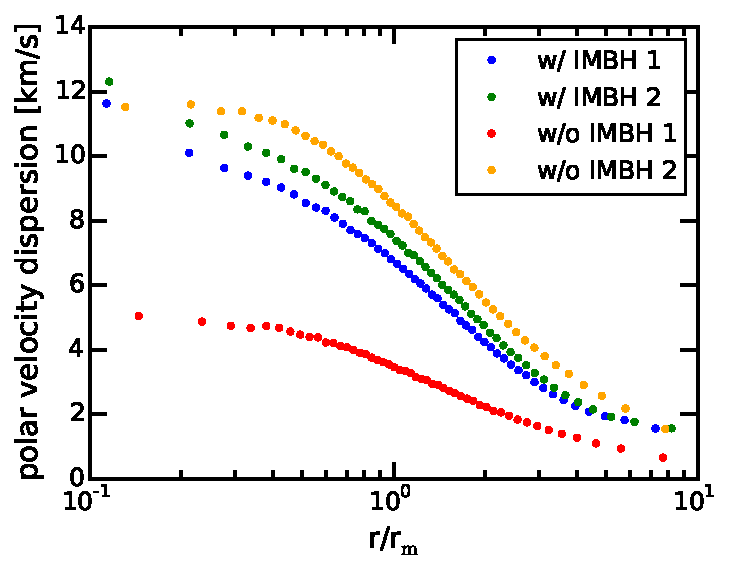
\includegraphics[width=\textwidth]{Plots/polar_velocity_dispersion.pdf}
		\caption{Polar velocity dispersions}
		\label{[fig:polar_vel_disp]}
	\end{subfigure}


	\caption{Velocity dispersion profiles of \(\mathrm{v_r, v_\phi,v_\theta}\) as a function of the radius in units of the half-mass radius \(\mathrm{r_{m}}\). Blue and green points are the velocity dispersions of SIM 1 and 2 and the red and yellow ones are the velocity dispersions of SIM 3 and 4. They are binned in a way that each bin contains the same amount of stars. The given radius is the mean radius of the stars of each bin. We can see that the velocity dispersion of the simulations with \ac{IMBH} rises towards the centre whereas the simulations without \ac{IMBH} exhibits a cored profile.}
	\label{fig:vel_disp}
\end{figure*}
As expected there is a rise in the centre for the simulations with \ac{IMBH}. This is due the high gravitational potential of the \acp{IMBH} which disturbs the dynamics of close stars. The rise is equally visible in all three velocity components. This is since the kinematics are isotropic in the centre of the \ac{GC} (see figure \ref{fig:anisotropy_param}). There is no difference in the polar and the azimuthal velocity dispersion profiles because the system is spherical. In the outer regions the radial velocity dispersion decreases linear while the tangential slope becomes less steep. The motion in the outer angular shells seems to be different to the motion in radial direction.



\par In \ref{fig:vel_disp} we noted a difference in the radial and in the tangential velocity dispersion. To properly quantify that difference we consider the anisotropy profile. Anisotropy can be calculated from equation \eqref{eq:anisotropy} in \ref{kin_prof_theory}.  Radial anisotropy means that there is higher velocity dispersion in radial direction than in angular direction. This comes probably along with a substantial number on eccentric orbits. The profile is binned the same way as the velocity dispersions and given in units of the half-mass radius.
\begin{figure}[htbp]
	\centering
	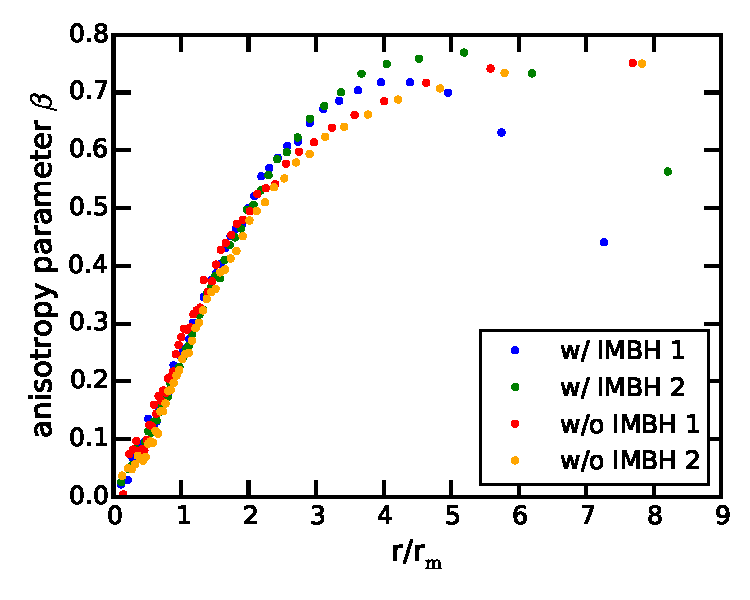
\includegraphics[width=0.475\textwidth]{Plots/anisotropy_parameter_beta.pdf}
	\caption{Profile of the anisotropy parameter \(\beta\). The colors are given as in \ref{fig:vel_disp}. All simulations are isotropic in the centre and become increasingly radial anisotropic in the intermediate regions. The simulations with \acp{IMBH} have a peak at 4 and 5 effective radii where they are most radial anisotropic. Some difference in anisotropy is observable between the simulations with and without \ac{IMBH}. This is due to different truncation prescriptions used in the simulations. We note that within \(\approx 2\mathrm{r_m}\) all simulations exhibit the same anisotropy profile.}
	\label{fig:anisotropy_param}
\end{figure}
In the central \(\approx 2\mathrm{r_m}\) of all \acp{GC} there is nearly the same anisotropy: isotropy in the centre \& radial anisotropy while going in the outer parts. That means the systems are radial anisotropic. In the centre the anisotropy is zero. There the system is isotropic and the stars move in no preferred direction. The \acp{GC} with \ac{IMBH} are most radially anisotropic at about 4 effective radii. The other \acp{GC} are becoming more radial anisotropic the further away from the centre it is. The difference is due to different truncation prescriptions of the simulation.

\subsubsection{Spatial distribution}
It is important to determine the density distribution for several reasons:
\begin{itemize}
\item[It is interesting to see if the simulated \acp{GC} habe radial density profiles that are similar to each other]
\item[and to classical \acp{GC} profiles like the Plummer potential (see section \ref{sec:other_pot})]
\item 

\end{itemize}The density profile shows the density calculated by equation \eqref{eq:density} of the system over its radius. As bins we use radial shells with logarithmic spacing chosen so that they are at least 100 stars per bin to have a reliable statistic. Outside of the cluster the density is set to 0. In the centre of the \acp{GC} (the distance of the 300th star of each simulation) we extrapolate the density profiles by setting it to the constant value of the innermost shell. 

\begin{figure}[htbp]
	\centering
	\begin{subfigure}{0.475\textwidth}
		\centering
		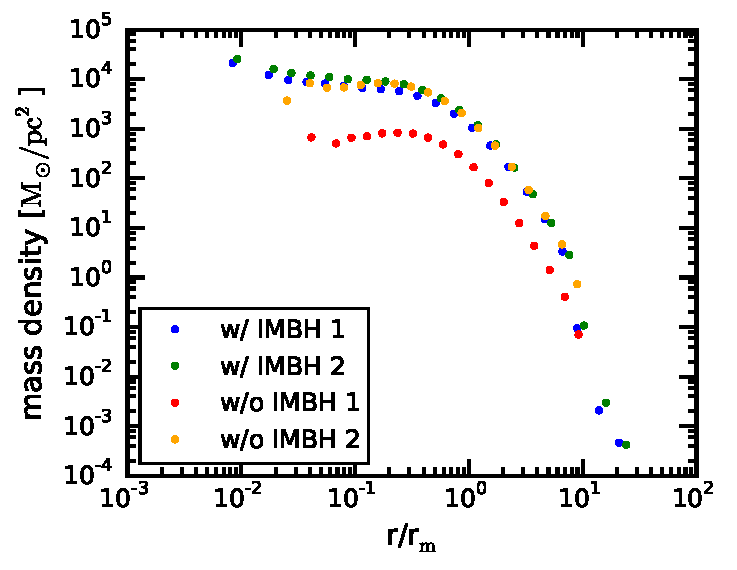
\includegraphics[width=\textwidth]{Plots/density_profiles.pdf}
		\caption{Mass density profiles of all four simulations.}
		\label{fig:mass_dens_points}
	\end{subfigure}
	\hfill
	\begin{subfigure}{0.475\textwidth}
		\centering
		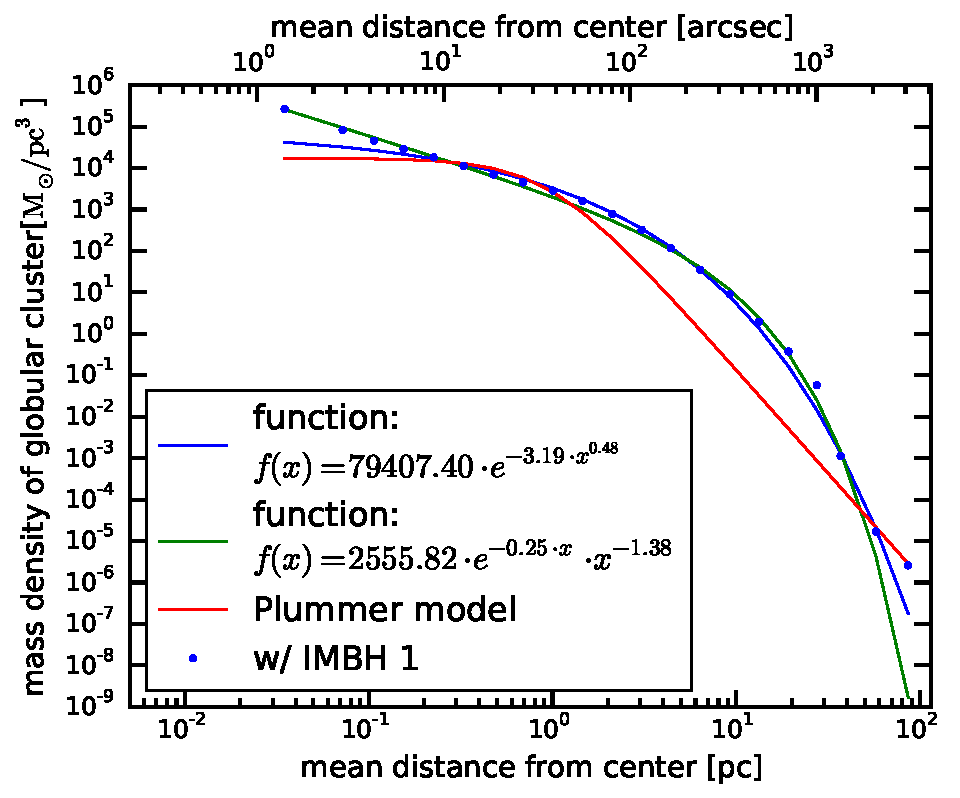
\includegraphics[width=\textwidth]{Plots/density_prof_analytic.pdf}
		\caption{Analytically fitted mass density profile of SIM 1.}
		\label{fig:mass_dens_ana}
	\end{subfigure}
	\vskip\baselineskip
	\begin{subfigure}{0.475\textwidth}
		\centering
		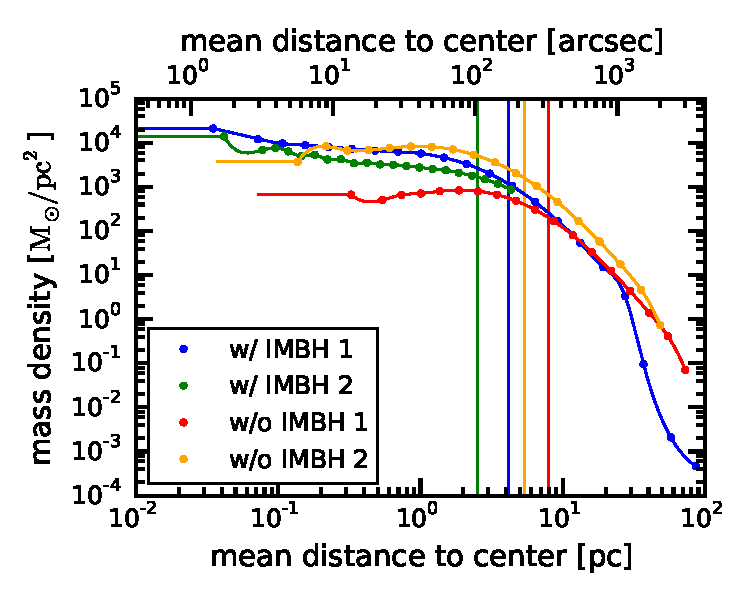
\includegraphics[width=\textwidth]{Plots/density_profiles_interpolated.pdf}
		\caption{Interpolated mass density profiles of SIM 1 and SIM 3.}
		\label{fig:mass_dens_intpol}
	\end{subfigure}
	\caption{Mass density profiles. The density in \(\frac{M_{\odot}}{pc^2}\) is plotted against the effective radius. The density of the \ac{GC} with \ac{IMBH} is everywhere larger than the density of the \ac{GC} without \ac{IMBH}. In the centre there is a raise in the density of the \ac{GC} with \ac{IMBH} whereas the other \ac{GC} stays approximately on the same level. Both start decreasing at about 0.5 \(\mathrm{r_eff}\). We can see in Panel \ref{fig:mass_dens_intpol} that it is not simple to find an analytical function describing the density globally for both low \& high radius. That is why we interpolate it in Panel \ref{fig:mass_dens_intpol}. Everything out of the \ac{GC} is set to 0 while the innermost density is set to be the value of the innermost point.}
	\label{fig:mass_density_profile}
\end{figure}
We try to find a analytic fitting function to the density profile for SIM 1 to calculate the potential from the Poisson's equation \eqref{eq:Poisson}. We use two variations of an exponential function which could fit well. Also we want to check if the density follows a classical \ac{GC} profile which i.e. is the Plummer profile. In Figure \ref{fig:mass_dens_ana} we see that we can not find a simple fitting function nor a classical profile which describes the density. To get a analytical function we continue by using the interpolated density given in Figure \ref{fig:mass_dens_intpol}.

\par We test the sphericity of the \ac{GC} and its \ac{COM}. Sphericity allows the usage of analytical methods that are very straight forward, especially for determing the potential of the globular cluster and from that the actions in action space. We will do this by splitting the \ac{GC} into octants and compare their mass density profiles. As one can see they're acceptable overlaying \color{red} within their errors \color{black}. This is done first for the centre of the coordinate system. We do the same for the centre of mass which is calculated by formula \color{red} insert formula in theory part somewhere \color{black} and compare it in figure \ref{fig:sphericity_com}.
\begin{figure}[htbp]
\centering
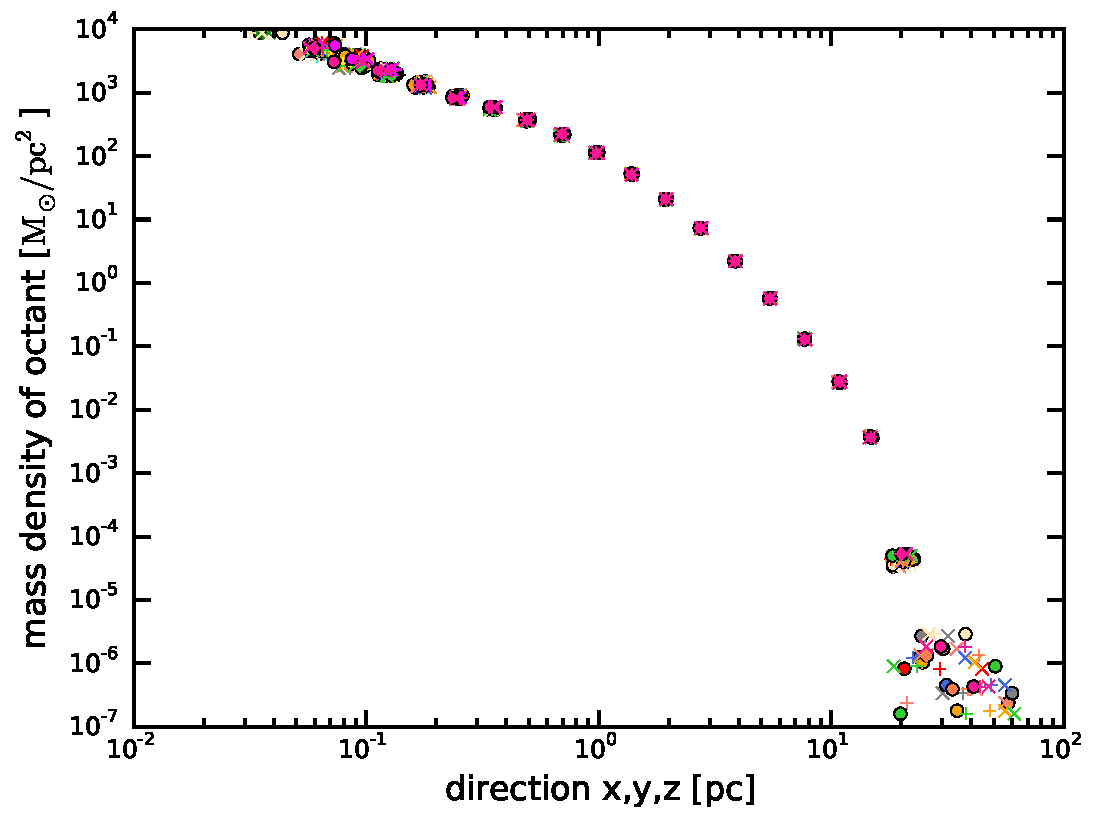
\includegraphics[width=0.7\textwidth]{Plots/sphericity_com.pdf}
\caption{Test for sphericity and center of mass of SIM 1.}
\label{fig:sphericity_com}
\end{figure}

\par From the density profile we can compute the potential as described in \ref{dens_pot_theory}. It is composed by the potential given from the stars and if there is one the potential of the \ac{IMBH} expressed as Kepler potential.
\begin{figure}[htbp]
	\centering
	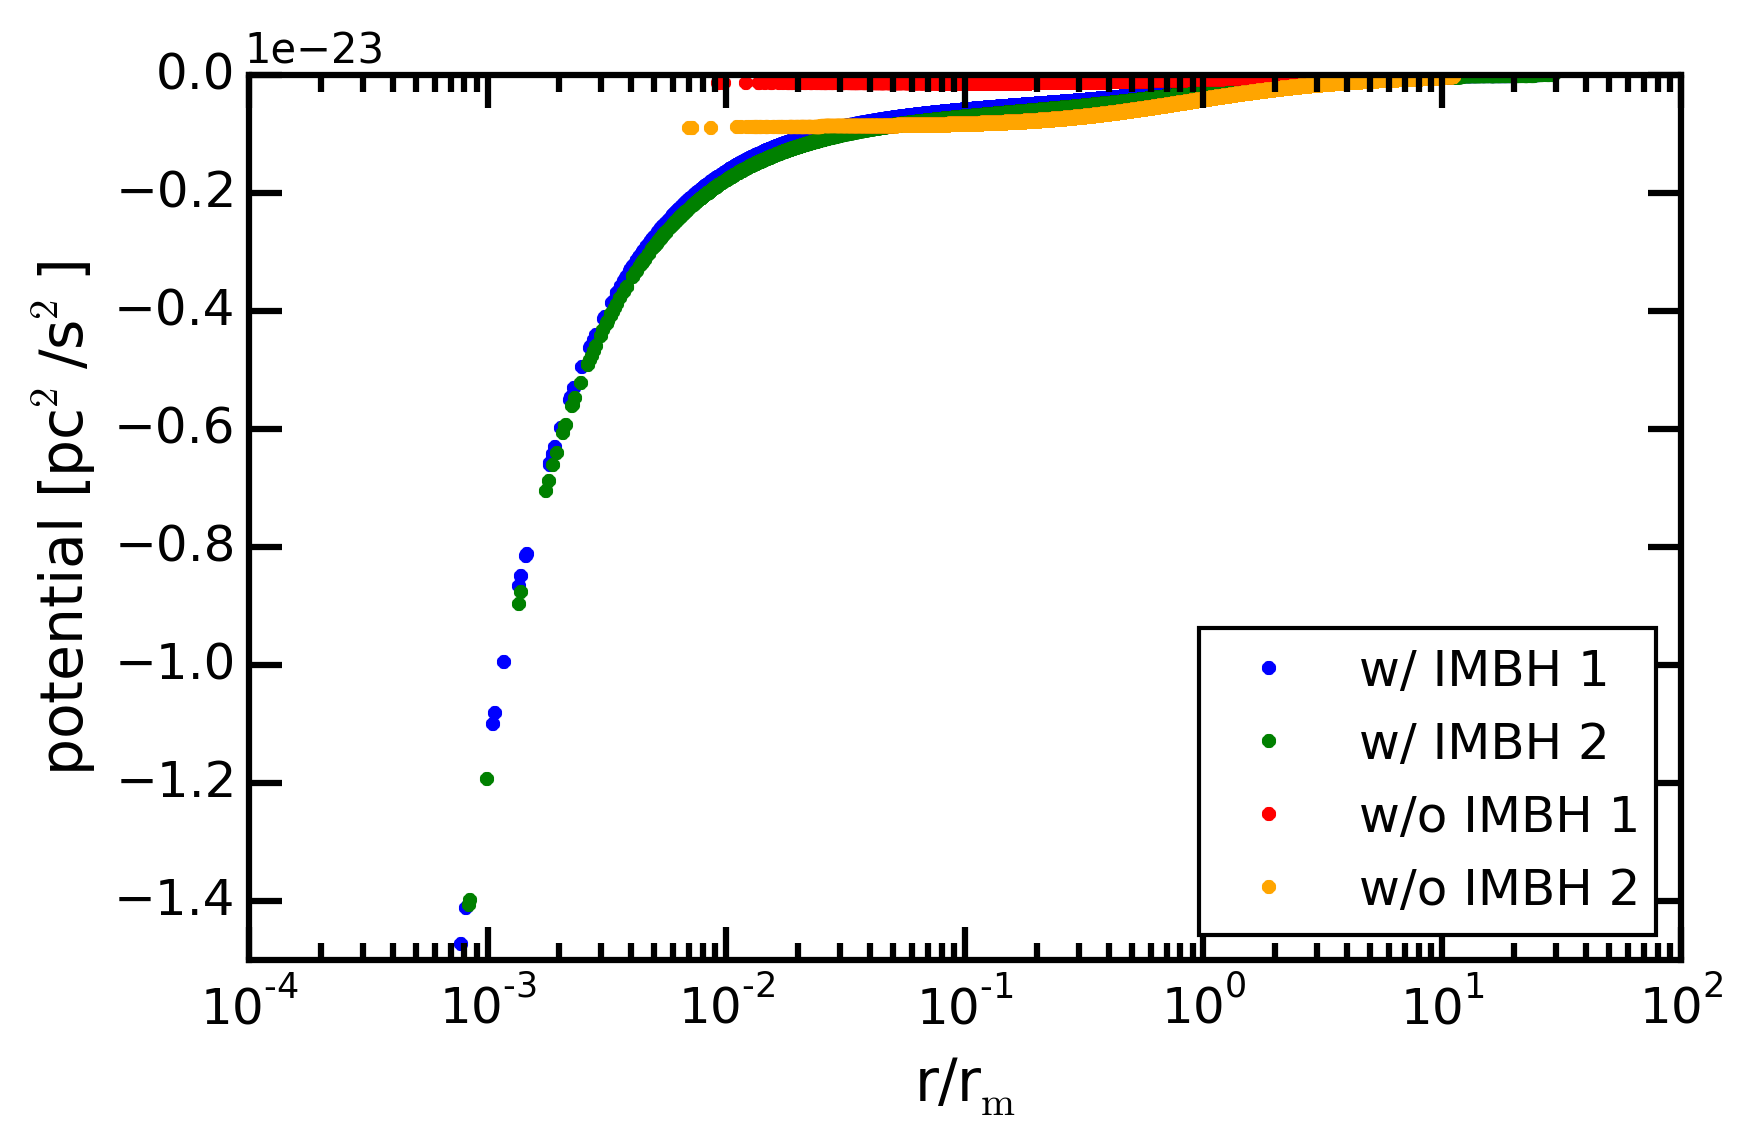
\includegraphics[width=0.475\textwidth]{Plots/potential.png}
	\caption{Potential of all \acp{GC}. SIM 1 and SIM 2 are nearly overlaying. They are the same simulation at different ages. The simulation lost 5 \% of its stars with 10 \% of the total mass while the \ac{IMBH} gained 13 \%. The potential of the stars declines while the potential of the \ac{IMBH} rises so the potential stays the same. The \acp{GC} without \ac{IMBH} remain constant in the inner part (until 0.5 half mass radii) and decrease from the points where their densities decrease.}
\end{figure}


\subsection{Investigations in action space}
After investigating the orbits at given actions and the time evolution of the integrals of motion we consider all actions and other integrals of motion at our given snapshots. We have a look at the energies and angular momenta of the stars and compare them with the radial actions. Our main goal is to find any systematic signatures for the simulations with \acp{IMBH} that can be considered as the direct evidence of the dynamical effect of the \ac{IMBH} itself. For this reason we investigate selected stars which show an abnormal behaviour in above-mentioned plots and compare them to the rest of the data to see where we find them.
\subsubsection{Energy}
\begin{figure}[htbp]
\centering
	\begin{subfigure}{0.475\textwidth}
		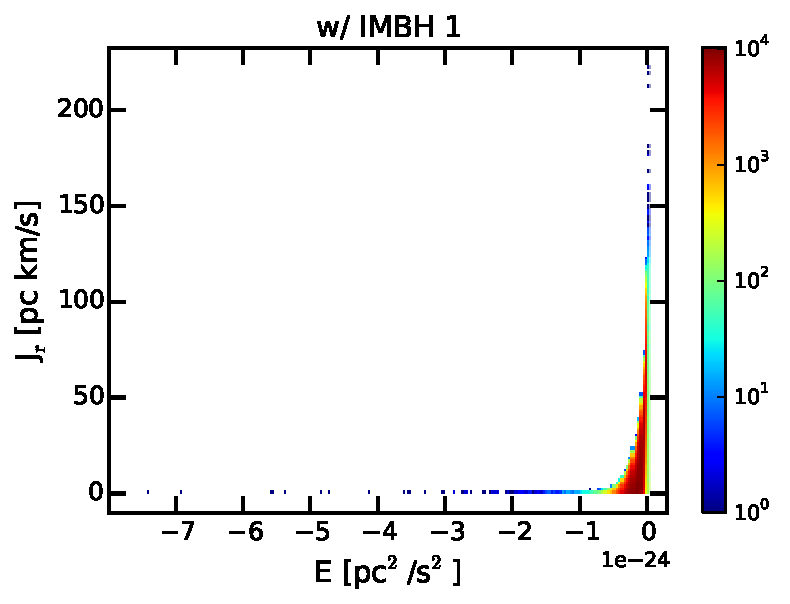
\includegraphics[width=\textwidth]{Plots/E_J_r_hist_IMBH1.pdf}
		\caption{SIM 1}
		\label{fig:E_J_r_hist_IMBH1}
	\end{subfigure}
	\hfill
	\begin{subfigure}{0.475\textwidth}
		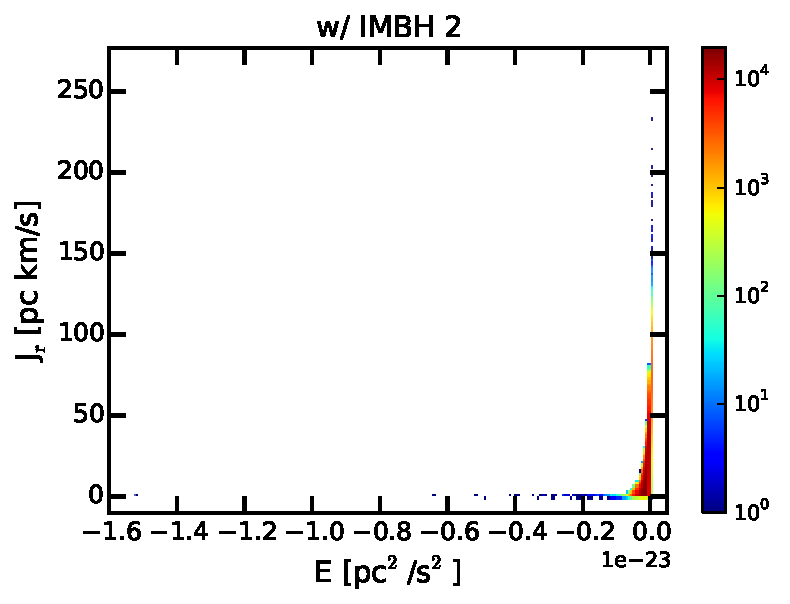
\includegraphics[width=\textwidth]{Plots/E_J_r_hist_IMBH2.pdf}
		\caption{SIM 2}
		\label{fig:E_J_r_hist_IMBH2}
	\end{subfigure}
	\vskip\baselineskip
	\begin{subfigure}{0.475\textwidth}
		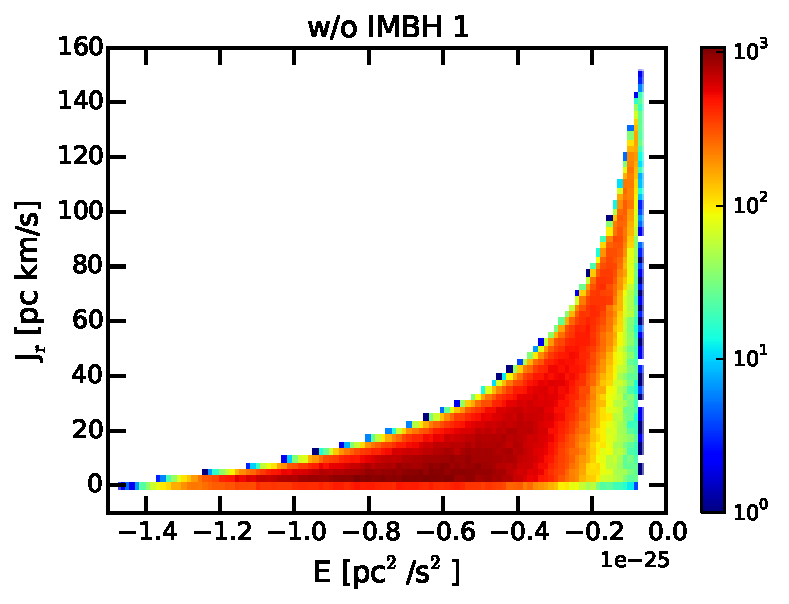
\includegraphics[width=\textwidth]{Plots/E_J_r_hist_noIMBH1.pdf}
		\caption{SIM 3}
		\label{fig:E_J_r_hist_noIMBH1}
	\end{subfigure}
	\hfill
	\begin{subfigure}{0.475\textwidth}
		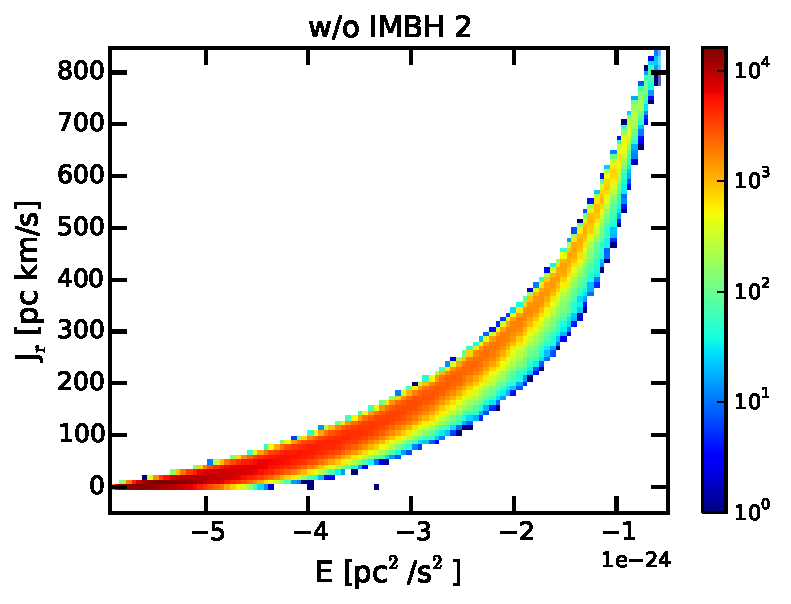
\includegraphics[width=\textwidth]{Plots/E_J_r_hist_noIMBH2.pdf}
		\caption{SIM 4}
		\label{fig:E_J_r_hist_noIMBH2}
	\end{subfigure}
	\caption{Radial action over energy. In \ref{fig:E_J_r_hist_IMBH1} and \ref{fig:E_J_r_hist_IMBH2} it is plotted for both simulations with \ac{IMBH} and the lower ones are for the simulation without \ac{IMBH}. We find the crescent shape from \ref{fig:E_J_r_hist_noIMBH1} and \ref{fig:E_J_r_hist_noIMBH2} clearly in \ref{fig:E_J_r_hist_IMBH1} and \ref{fig:E_J_r_hist_IMBH2}. But in SIM 1 and SIM 2 there are some stars differing from this shape. Some have high energy with no radial actions (henceforth referred to as group 1) while others have high radial actions with nearly no energy (henceforth group 2).}
	\label{fig:E_J_r_hist}
\end{figure}	
In \ref{fig:E_J_r_hist} we plot the radial action over the energy of the star as histograms for all \acp{GC}. We see clearly some stars outside of the moon shape. They have either no radial action and high energy(below \(-4 \cdot10^{-24}\) \(pc^2/s^2\)) or nearly no energy and high radial action (above 500 pc km/s). 

\par We check the effective potential of the stars of the group to get information of their orbits and their actual positions. In \ref{fig:eff_pot} show one exemplary graph for each group taken from SIM 1. 

\begin{figure}
\centering
	\begin{subfigure}{0.475\textwidth}
	\centering
	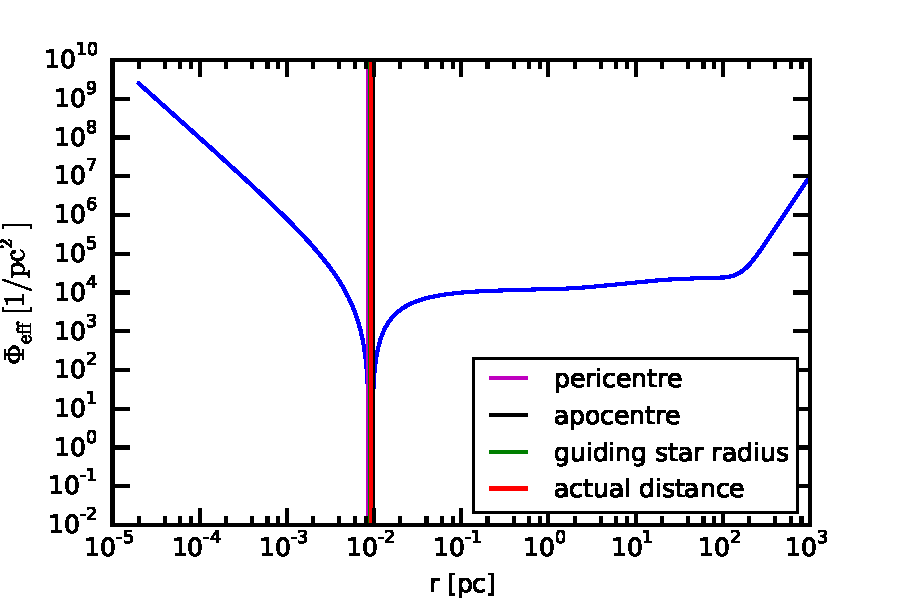
\includegraphics[width=\textwidth]{Plots/pot_eff_group1.pdf}
	\caption{Star of group 1}
	\label{fig:pot_eff_group1}
	\end{subfigure}
	\hfill
	\begin{subfigure}{0.475\textwidth}
	\centering
	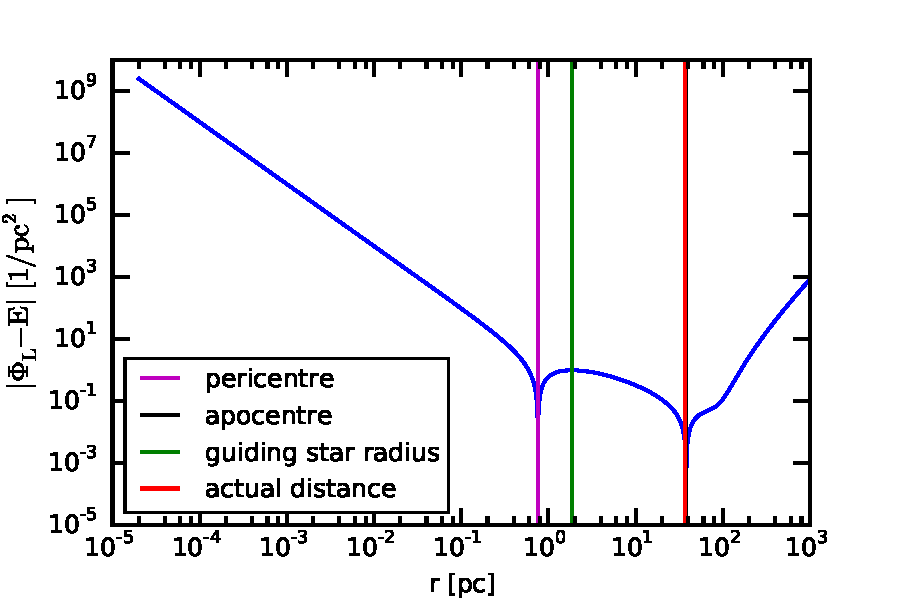
\includegraphics[width=\textwidth]{Plots/pot_eff_group2.pdf}
	\caption{Star of group 2}
	\label{fig:pot_eff_group2}
	\end{subfigure}	
\caption{Effective potential of exemplary stars of both groups from figure \ref{fig:E_J_r_hist}. The star of group 1 is clearly one a circular orbit with \(\mathrm{r_{min}\approx r_g\approx r \approx r_{max} }\). The star of group two has a highly eccentric orbit and its actual position is in its apocentre.}
\label{fig:eff_pot}
\end{figure}

\par The first group of stars of SIM 1 contains 38 of the nearest 110 stars including the innermost 15 stars. Since they have really low (nearly 0) radial actions they are on circular orbits. The nearest 15 on circular orbits around the \ac{IMBH} are certainly locked to the \ac{IMBH}. That is why we do not see this signature for SIM 3 and SIM 4. The other stars of this group are likely to be locked to the \ac{IMBH} as well while the rest of the near stars which are not in this group seem to be near to or in their pericentre on more elliptic orbits and therefore not locked to the \ac{IMBH}. 
\par The other group of stars with high radial actions and nearly no energy can not be clearly related to the \ac{IMBH}. They are the furthermost stars of the snapshot. All are in their apocentre on very elliptic orbits (\color{red} calculate ellipticity? \color{black}). This ellipticity could be caused by the \ac{IMBH} but since most of their pericentres are at a few pc we can not assume much interaction with the \ac{IMBH} for those stars. Another reason that these stars do not occur in this way in SIM 3 and SIM 4 can be due to different truncation prescriptions used in the simulations (see graph \ref{fig:anisotropy_param}). These stars are nearly outside of the \acp{GC} and have about zero energy so they could have been excluded in SIM 3 and SIM 4. 

\begin{figure}[htbp]
\centering
	\begin{subfigure}{0.475\textwidth}
		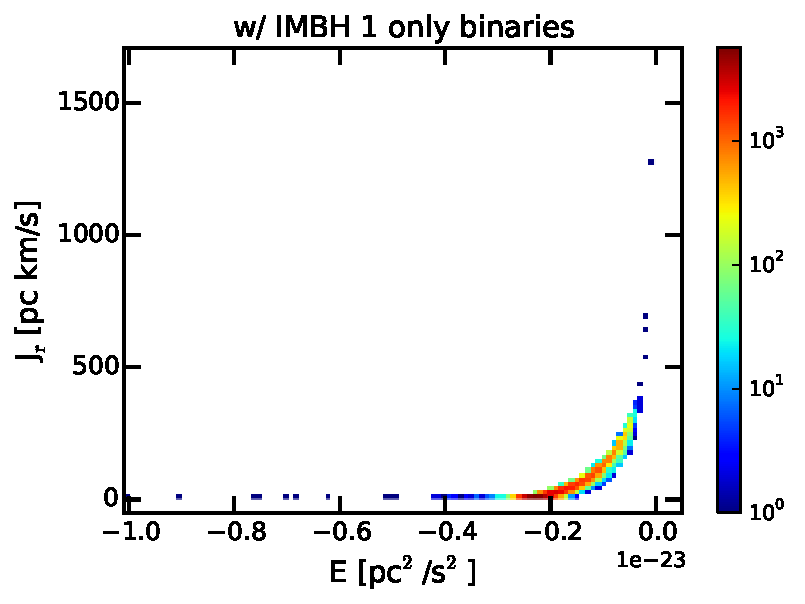
\includegraphics[width=\textwidth]{Plots/E_J_r_hist_bins_IMBH1.pdf}
		\caption{SIM 1}
		\label{fig:E_J_r_hist_bins_IMBH1}
	\end{subfigure}
	\hfill
	\begin{subfigure}{0.475\textwidth}
		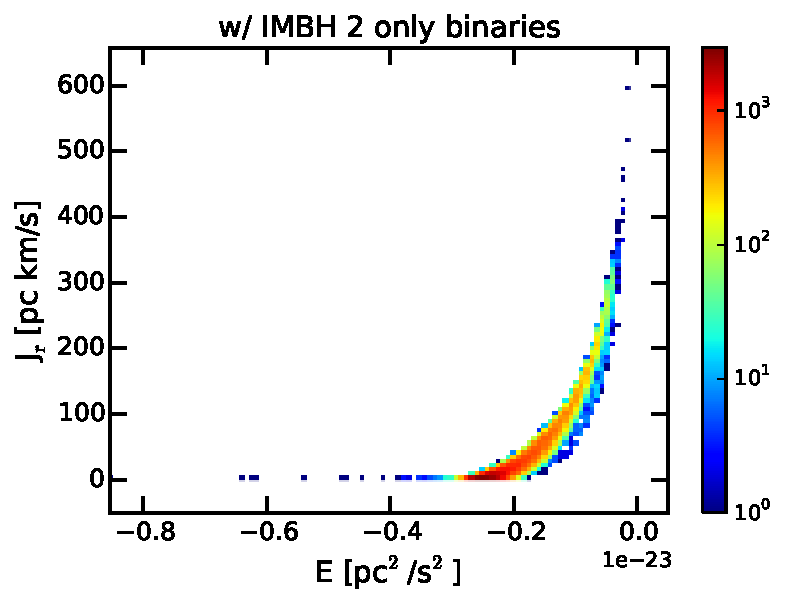
\includegraphics[width=\textwidth]{Plots/E_J_r_hist_bins_IMBH2.pdf}
		\caption{SIM 2}
		\label{fig:E_J_r_hist_bins_IMBH2}
	\end{subfigure}
	\vskip\baselineskip
	\begin{subfigure}{0.475\textwidth}
		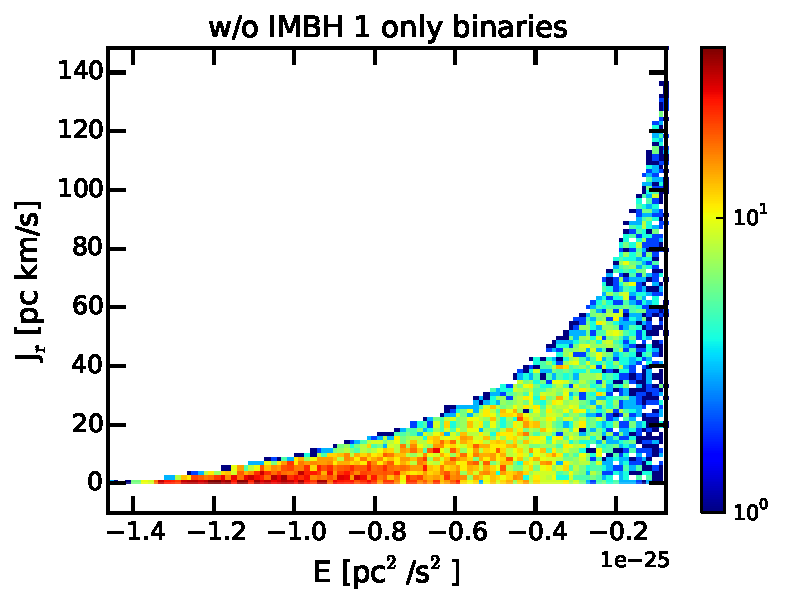
\includegraphics[width=\textwidth]{Plots/E_J_r_hist_bins_noIMBH1.pdf}
		\caption{SIM 3}
		\label{fig:E_J_r_hist_bins_noIMBH1}
	\end{subfigure}
	\hfill
	\begin{subfigure}{0.475\textwidth}
		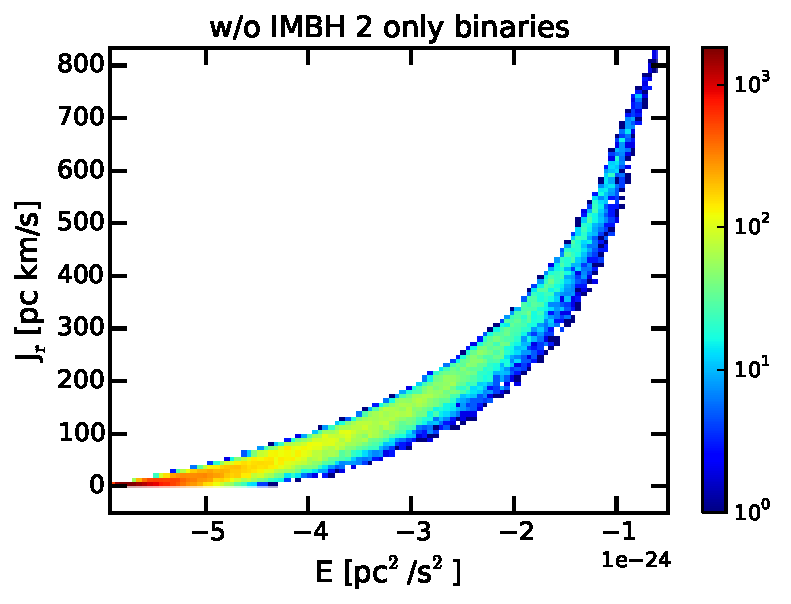
\includegraphics[width=\textwidth]{Plots/E_J_r_hist_bins_noIMBH2.pdf}
		\caption{SIM 4}
		\label{fig:E_J_r_hist_bins_noIMBH2}
	\end{subfigure}
	\caption{Radial action over energy only of binary systems. We see the same distribution of stars as in \ref{fig:E_J_r_hist}.}
	\label{fig:E_J_r_bins_hist}
\end{figure}

\par We might get these high energies from former binaries which were divided earlier. One of the stars could have been captured on a circular orbit near the centre while the other could have been left on an unbound orbit and have left the system. To check this we will plot the same values only for our actual binary systems. As we see in \ref{fig:E_J_r_bins_hist} the binary systems are behaving like single stars. There is no signature that the divergent stars are leftovers of former binaries. 

\subsubsection{Angular momentum}
\begin{figure}[htbp]
\centering
	\begin{subfigure}{0.475\textwidth}
		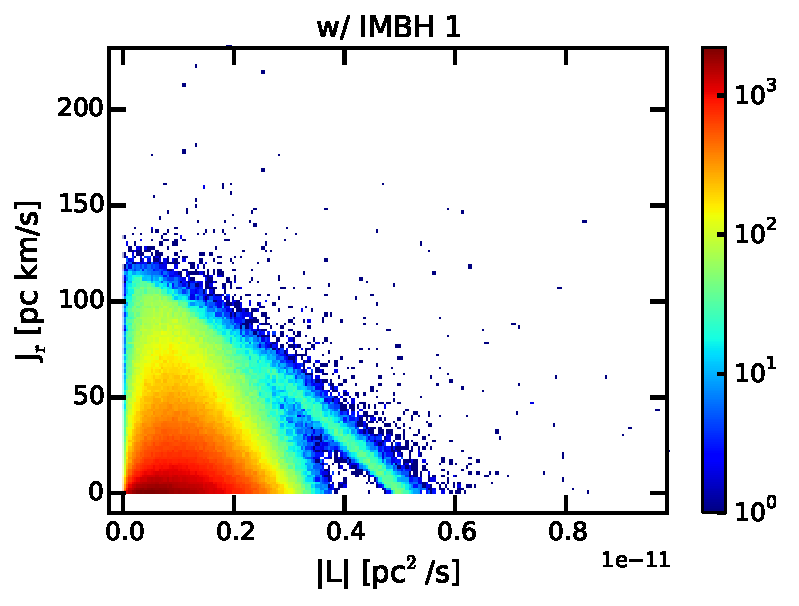
\includegraphics[width=\textwidth]{Plots/L_J_r_hist_IMBH1.pdf}
		\caption{SIM 1}
		\label{fig:L_J_r_hist_IMBH1}
	\end{subfigure}
	\hfill
	\begin{subfigure}{0.475\textwidth}
		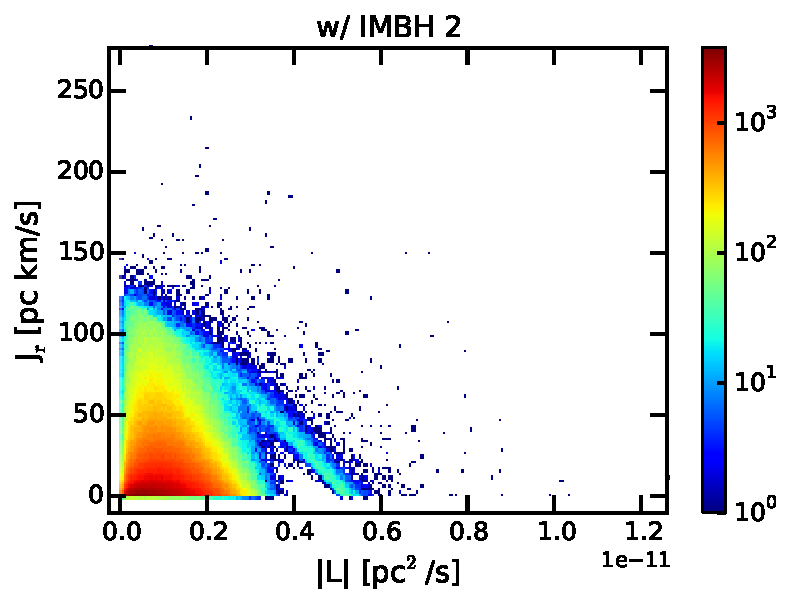
\includegraphics[width=\textwidth]{Plots/L_J_r_hist_IMBH2.pdf}
		\caption{SIM 2}
		\label{fig:L_J_r_hist_IMBH2}
	\end{subfigure}
	\vskip\baselineskip
	\begin{subfigure}{0.475\textwidth}
		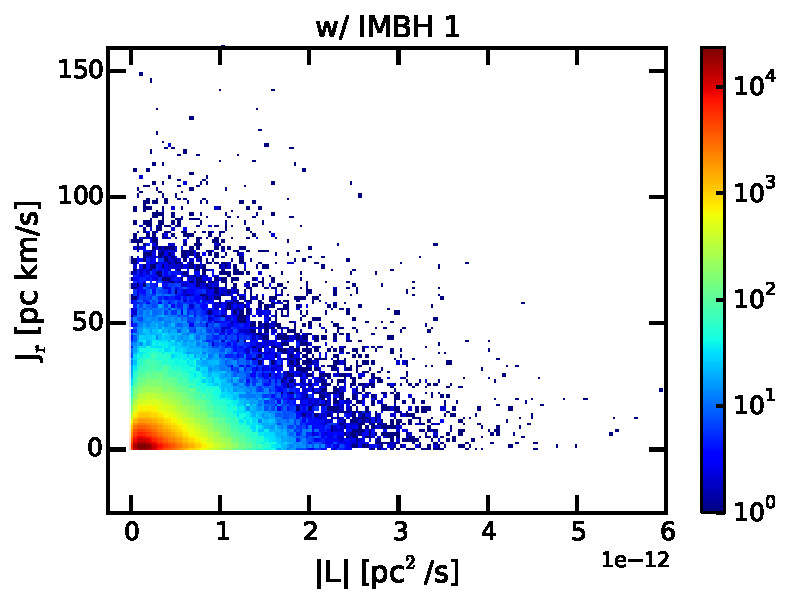
\includegraphics[width=\textwidth]{Plots/L_J_r_mass_hist_IMBH1.pdf}
		\caption{SIM 1 mass weighted}
		\label{fig:L_J_r_mass_hist_IMBH1}
	\end{subfigure}
	\hfill
	\begin{subfigure}{0.475\textwidth}
		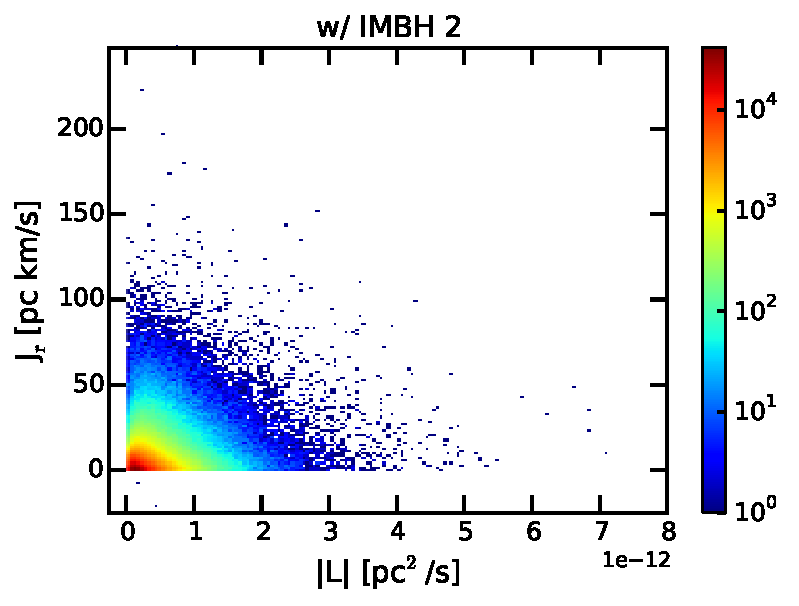
\includegraphics[width=\textwidth]{Plots/L_J_r_mass_hist_IMBH2.pdf}
		\caption{SIM 2 mass weighted}
		\label{fig:L_J_r_mass_hist_IMBH2}
	\end{subfigure}
	\vskip\baselineskip	
	\begin{subfigure}{0.475\textwidth}
		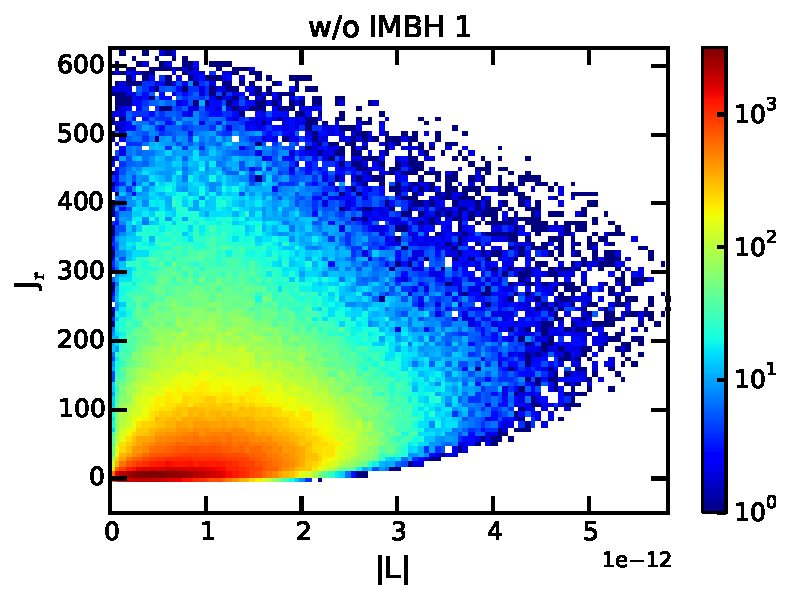
\includegraphics[width=\textwidth]{Plots/L_J_r_hist_noIMBH1.pdf}
		\caption{SIM 3}
		\label{fig:L_J_r_hist_noIMBH1}
	\end{subfigure}
	\hfill
	\begin{subfigure}{0.475\textwidth}
		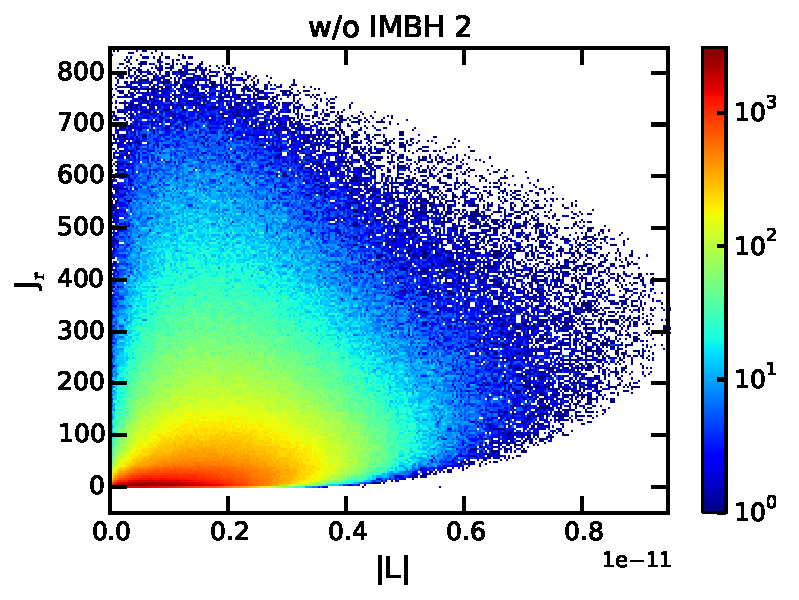
\includegraphics[width=\textwidth]{Plots/L_J_r_hist_noIMBH2.pdf}
		\caption{SIM 4}
		\label{fig:L_J_r_hist_noIMBH2}
	\end{subfigure}
	\caption{Radial action over angular momentum. \ref{fig:L_J_r_hist_noIMBH1} and \ref{fig:L_J_r_hist_noIMBH2} look again very similar to each other with no recognizable substructure. In \ref{fig:L_J_r_hist_IMBH1} and \ref{fig:L_J_r_hist_IMBH2} there are stars above the main shape. In the shape we can clearly see a substructure from about 0.3 to about 0.5 pc\(^2\)/s in nearly the whole radial action range. \color{red}half moon not directly spatially connected to imbh (plot mit color coding pericentre einfügen) probably only specific to the simulation\color{black}}
	\label{fig:L_J_r_hist}
\end{figure}

\begin{figure}[htbp]
\centering
	\begin{subfigure}{0.475\textwidth}
	\centering
	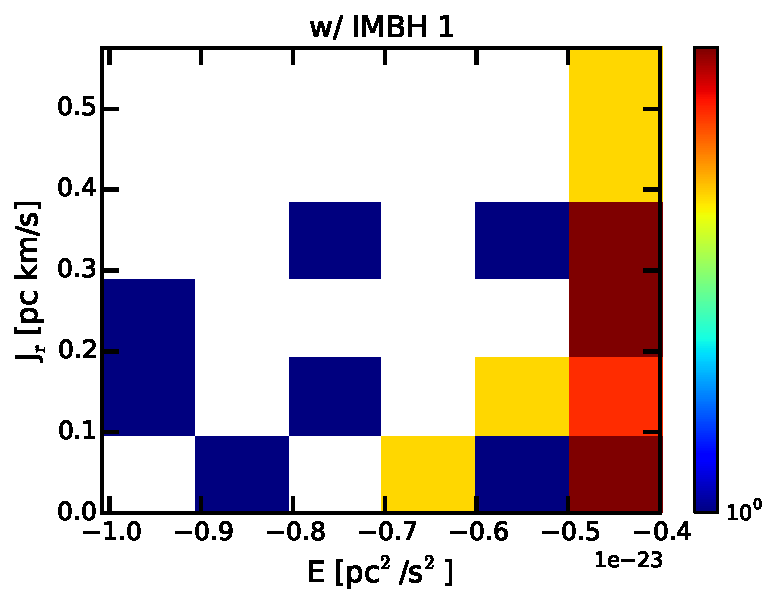
\includegraphics[width=\textwidth]{Plots/E_J_r_justIMBH_hist_IMBH1.pdf}
	\caption{Radial action over energy only for \ac{IMBH} influenced stars of SIM 1.}
	\label{fig:E_J_r_justIMBH_1}
	\end{subfigure}
	\hfill
	\begin{subfigure}{0.475\textwidth}
	\centering
	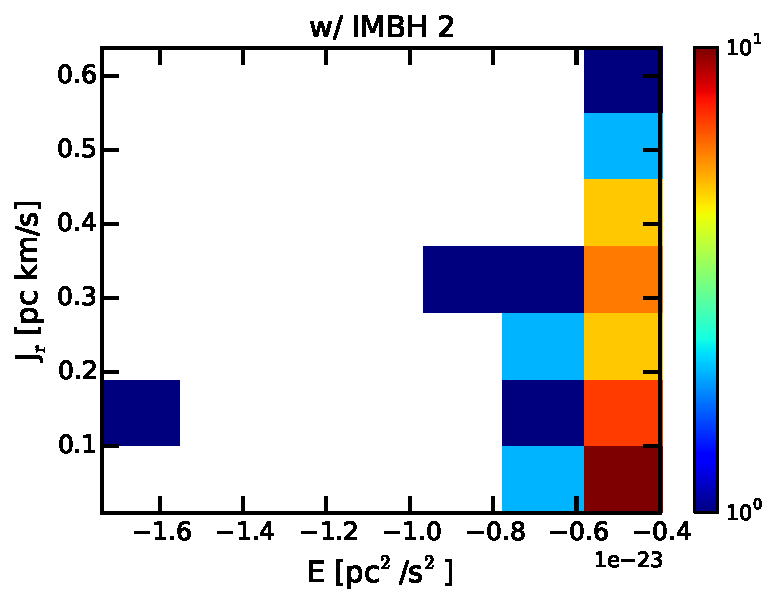
\includegraphics[width=\textwidth]{Plots/E_J_r_justIMBH_hist_IMBH2.pdf}
	\caption{Radial action over energy only for \ac{IMBH} influenced stars of SIM 2.}
	\label{fig:_E_r_justIMBH_2}
	\end{subfigure}	
	\vskip\baselineskip
	\begin{subfigure}{0.475\textwidth}
	\centering
	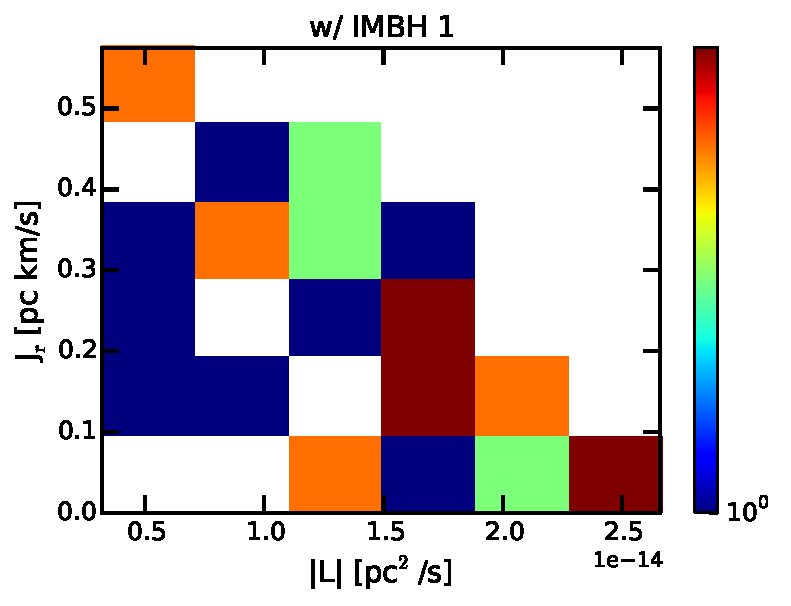
\includegraphics[width=\textwidth]{Plots/L_J_r_justIMBH_hist_IMBH1.pdf}
	\caption{Radial action over angular momentum only for \ac{IMBH} influenced stars of SIM 1.}
	\label{fig:L_J_r_justIMBH_1}
	\end{subfigure}
	\hfill
	\begin{subfigure}{0.475\textwidth}
	\centering
	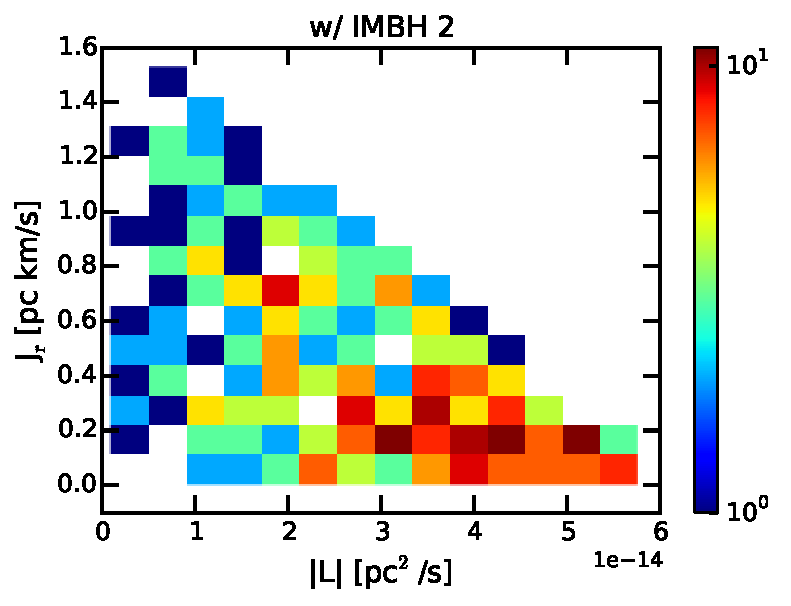
\includegraphics[width=\textwidth]{Plots/L_J_r_justIMBH_hist_IMBH2.pdf}
	\caption{Radial action over angular momentum only for \ac{IMBH} influenced stars of SIM 2.}
	\label{fig:L_J_r_justIMBH_2}
	\end{subfigure}	
\caption{Check for group 1 stars.}
\label{fig:just_IMBH_hist}	
\end{figure}
\par Next we plot the radial actions over the absolute angular momenta of the stars of the simulations again as histograms. In \ref{fig:L_J_r_hist} we can see a triangular shape which seems characteristic. Inside this shape we see some substructure in the \acp{GC} with \ac{IMBH}. The stars outside the shape are the stars of group 2 which we see in \ref{fig:E_J_r_hist} and \ref{fig:E_J_r_bins_hist} as the stars with no energy and high radial actions. Obviously they don't seem to have a specific angular momentum. We do not know how to identify the stars in the substructure. There could be a mass-dependent correlation due to dynamical mass segregation.

\subsubsection{Guiding star radius}
\par We extract these divergent stars and determine their properties. First we check the positions of their actions depending on their guiding star radii.
\begin{figure}[htbp]
\centering
	\begin{subfigure}{0.475\textwidth}
		\centering
		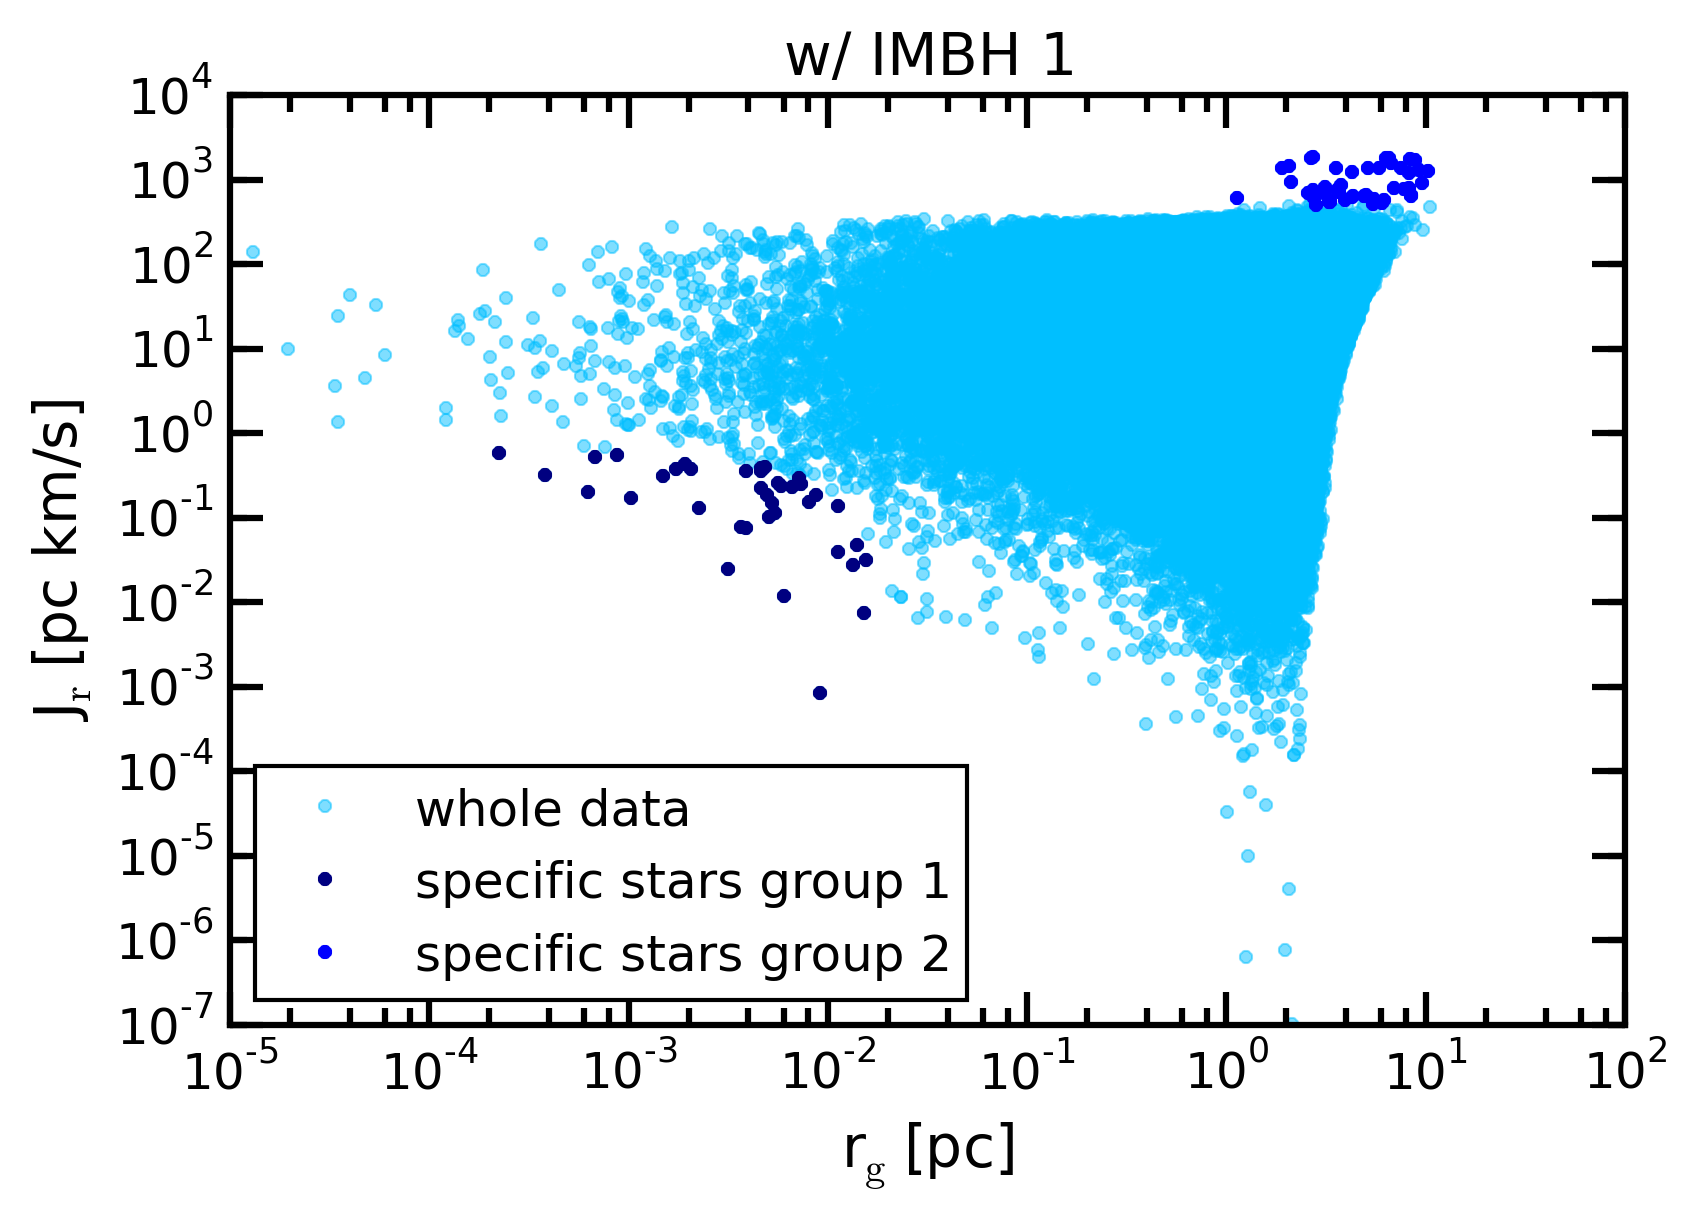
\includegraphics[width=\textwidth]{Plots/r_g_J_r_IMBH1.png}
		\caption{SIM 1}
		\label{fig:r_g_J_r_IMBH1}
	\end{subfigure}
	\hfill
	\begin{subfigure}{0.475\textwidth}
		\centering
		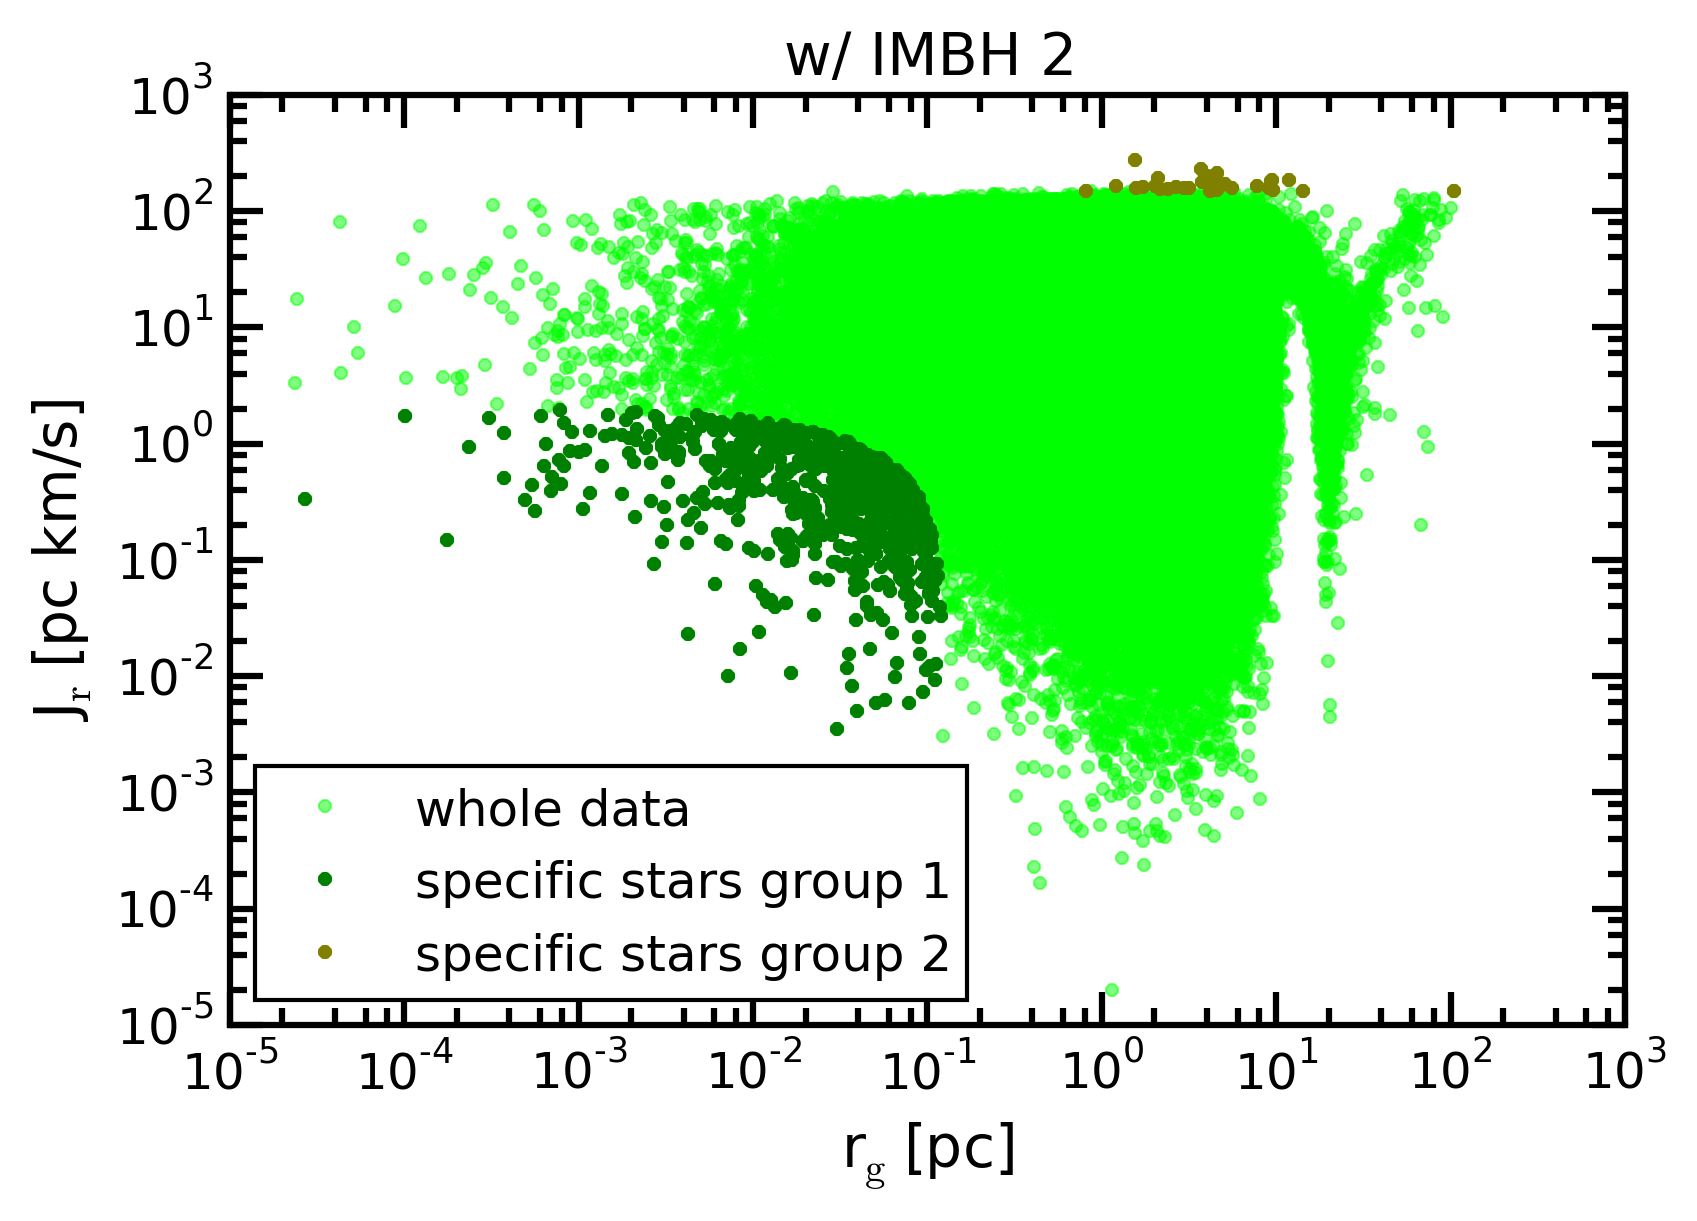
\includegraphics[width=\textwidth]{Plots/r_g_J_r_IMBH2.png}
		\caption{SIM 2}
		\label{fig:r_g_J_r_IMBH2}
	\end{subfigure}
	\vskip\baselineskip
	\begin{subfigure}{0.475\textwidth}
		\centering
		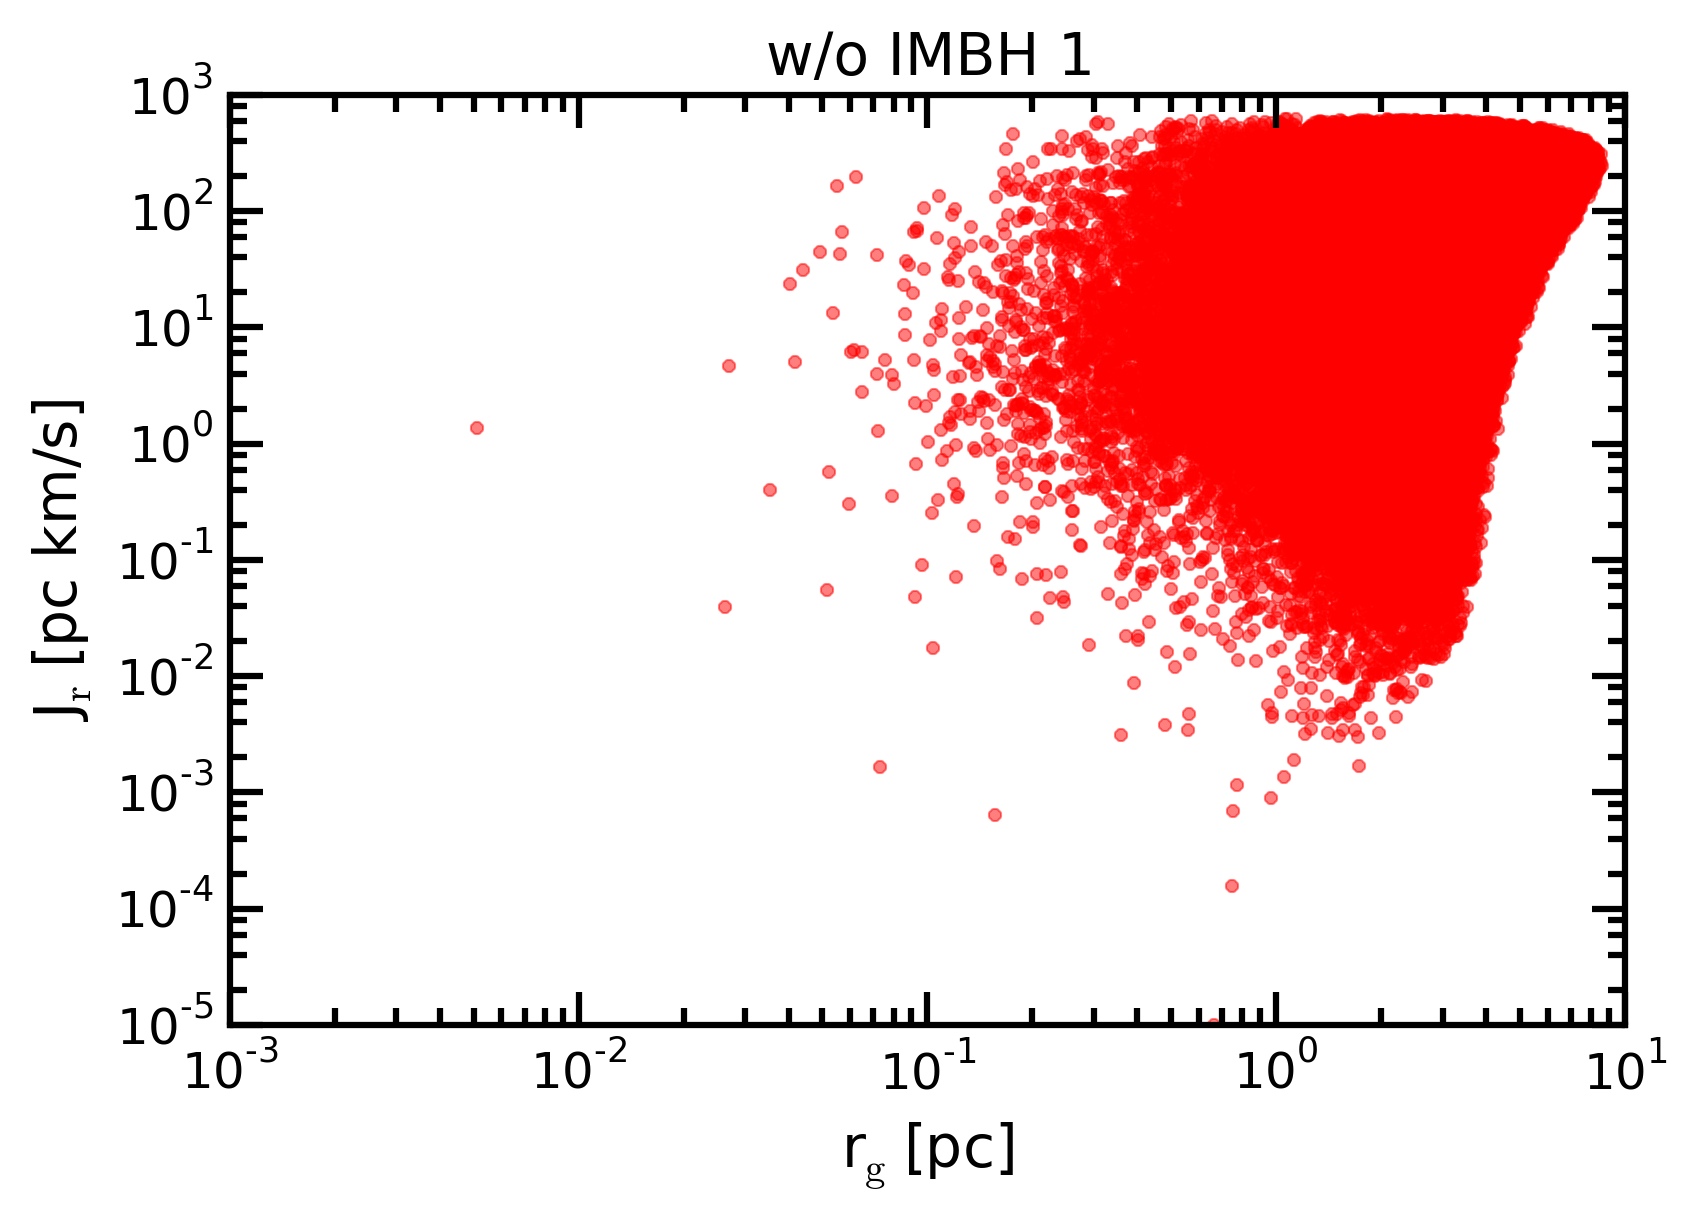
\includegraphics[width=\textwidth]{Plots/r_g_J_r_noIMBH1.png}
		\caption{SIM 3}
		\label{fig:r_g_J_r_noIMBH1}
	\end{subfigure}
	\hfill
	\begin{subfigure}{0.475\textwidth}
		\centering
		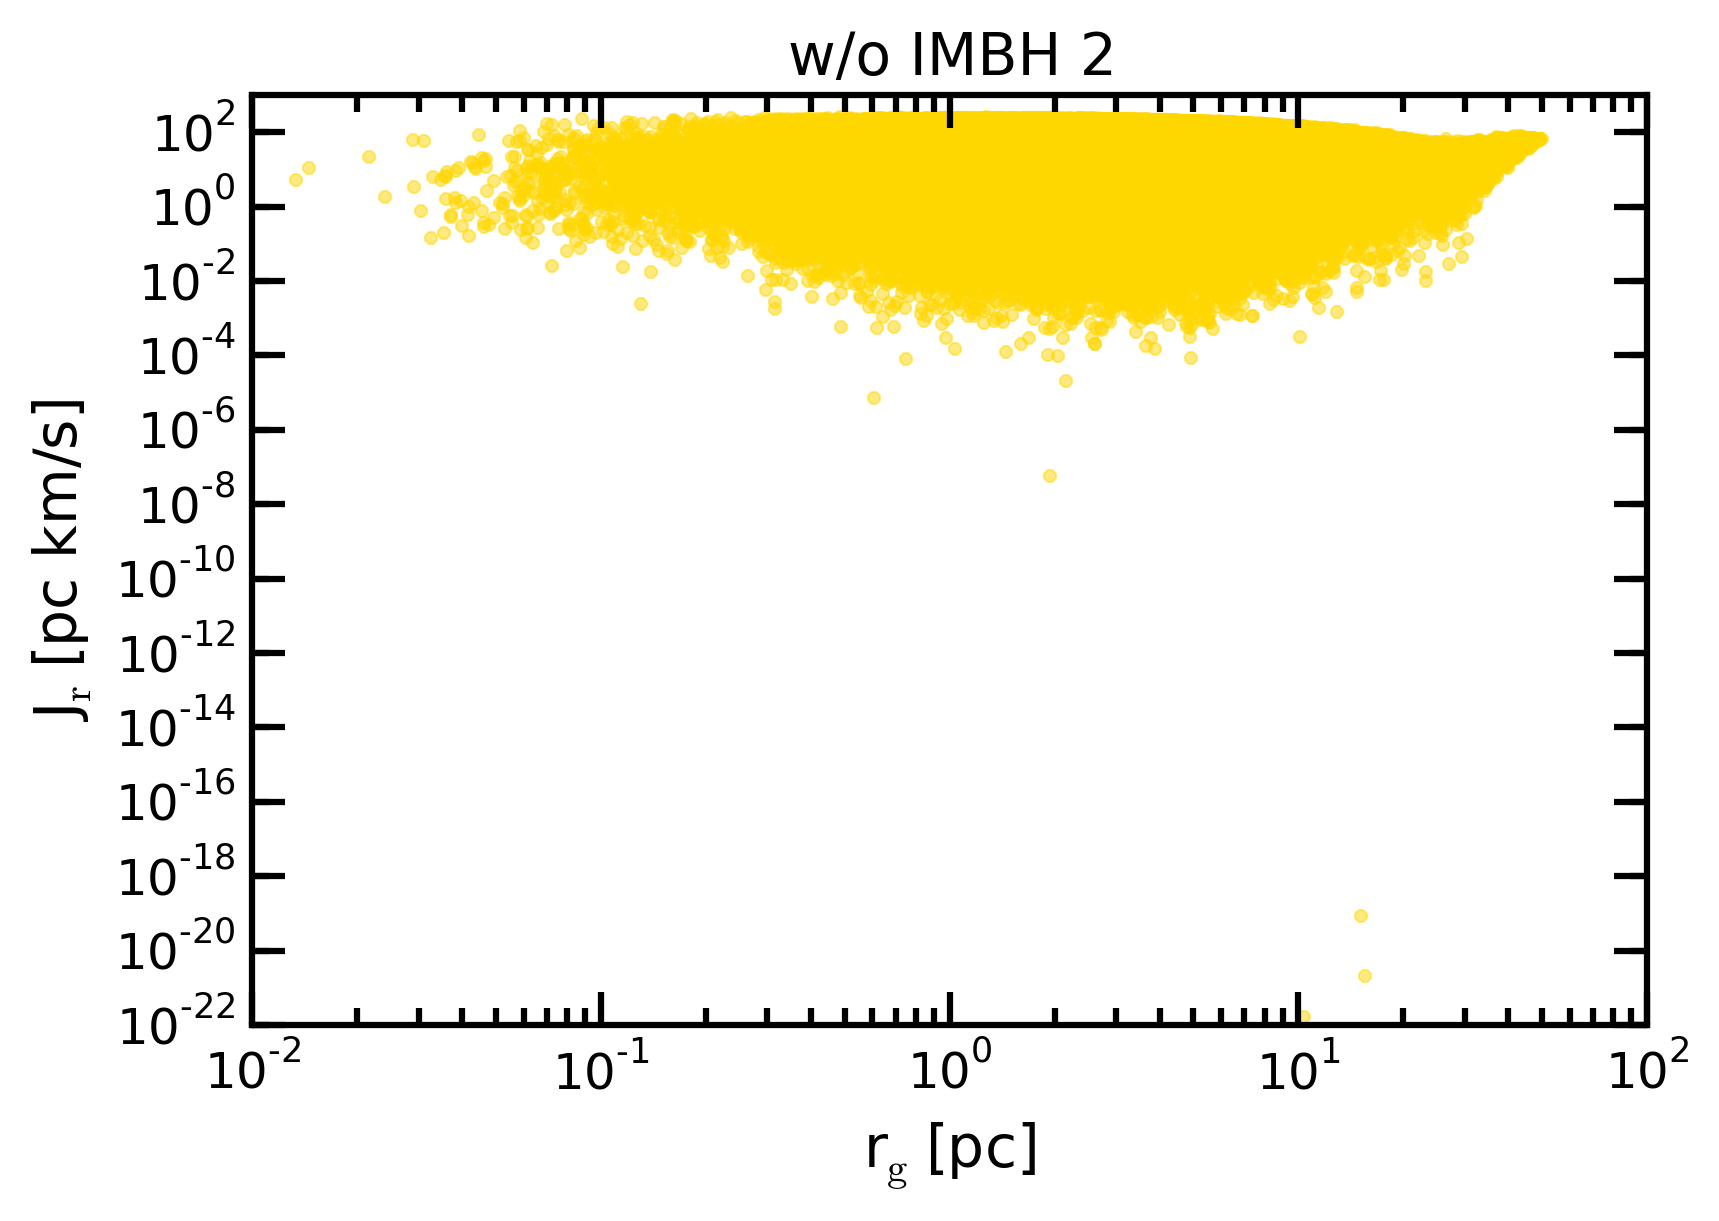
\includegraphics[width=\textwidth]{Plots/r_g_J_r_noIMBH2.png}
		\caption{SIM 4}
		\label{fig:r_g_J_r_noIMBH2}
	\end{subfigure}
	\caption{Radial action over guiding star radius with marked specific stars on loglog scale. All simulations have a similar shaped distributions except for the marked stars which are the specific ones. On the top right corner the shape of \ref{fig:E_J_r_hist_IMBH1} and \ref{fig:E_J_r_hist_IMBH2} is not gently rounded but there are single stars around it. On the lower left there are some extra stars which we identify as the stars with low radial action.}
	\label{fig:r_g_J_r}
\end{figure}
In graph \ref{fig:r_g_J_r} the radial actions are plotted over their guiding star distances. We highlight the stars of group 1 and group 2 taken from graph \ref{fig:E_J_r_hist} for SIM 1 and SIM 2. In general, there are several stars which have a really small guiding star radius (up to  \unit[\(10^-5\)]{pc}). In SIM 3 and SIM 4 only very few stars go below \unit[0.1]{pc}. Another difference between the \acp{GC} with and the ones without \ac{IMBH} is that on the right border the lower end goes until very low radial actions for SIM 1 and SIM 2 (up to \unitfrac[\(10^-6\)]{pc km}{s}) while SIM 3 and SIM 4 end there softly at about \unitfrac[\(10^-2\)]{pc km}{s}.

